% OpenTranscribe Performance Whitepaper
% Compile: pdflatex main.tex && pdflatex main.tex (two passes for floats)
\documentclass[conference,10pt]{IEEEtran}
\pagestyle{plain}

% -- Packages ------------------------------------------------------------------
\usepackage[T1]{fontenc}
\usepackage[utf8]{inputenc}
\usepackage{amsmath,amssymb}
\usepackage{booktabs}
\usepackage{multirow}
\usepackage{array}
\usepackage{tabularx}
\usepackage{siunitx}
\usepackage{xcolor}
\usepackage{pgfplots}
\usepackage{tikz}
\usepackage{float}
\usepackage{enumitem}
\usepackage{cite}
\usepackage[hyphens]{url}
\usepackage[bookmarks=false]{hyperref}

\pgfplotsset{compat=1.18}
\usetikzlibrary{shapes.geometric, arrows.meta, positioning, calc, fit, backgrounds}

% -- Color Definitions ---------------------------------------------------------
\definecolor{ieeeblue}{RGB}{0,84,147}
\definecolor{whispercolor}{RGB}{59,130,246}
\definecolor{pyannotecolor}{RGB}{239,68,68}
\definecolor{overheadcolor}{RGB}{156,163,175}
\definecolor{stockcolor}{RGB}{239,68,68}
\definecolor{optcolor}{RGB}{34,197,94}
\definecolor{vrambg}{RGB}{229,231,235}
\definecolor{idealcolor}{RGB}{156,163,175}

% -- SI Units Setup ------------------------------------------------------------
\sisetup{
  group-separator={,},
  group-minimum-digits=4,
  detect-weight=true,
}

% -- Custom column type --------------------------------------------------------
\newcolumntype{R}[1]{>{\raggedleft\arraybackslash}p{#1}}
\newcolumntype{C}[1]{>{\centering\arraybackslash}p{#1}}

% ==============================================================================
\begin{document}

\title{OpenTranscribe: GPU-Accelerated Transcription\\Pipeline Performance Analysis}

\author{
  \IEEEauthorblockN{David A. Macey}
  \IEEEauthorblockA{OpenTranscribe Project\\
    \url{https://github.com/davidamacey/OpenTranscribe}}
}

\maketitle

% ==============================================================================
% ABSTRACT
% ==============================================================================
\begin{abstract}
OpenTranscribe is an open-source self-hosted transcription platform that
combines GPU-accelerated speech recognition with speaker diarization. On an
NVIDIA RTX A6000, it processes a single file at \textbf{40.3$\times$ realtime}
and sustains 35--39$\times$ across durations from 30\,minutes to 4\,hours.
Thread-based concurrent GPU sharing scales linearly from 1 to 12 workers on a
single 48\,GB GPU, peaking at \textbf{54.6$\times$} aggregate throughput at
8 concurrent workers. A custom PyAnnote fork contributes a 1.28$\times$
diarization speedup with 66\% VRAM reduction and 115$\times$ lower CPU RAM
consumption. CTranslate2 \texttt{int8\_float16} quantization adds 20--30\%
to Whisper inference speed with $<$0.1\% WER degradation. With all GPU memory
leaks resolved, single-worker VRAM peaks at just 2.3\,GB---leaving 96\% of
the A6000 free for concurrent work. Against a production corpus of \num{1435}
files (\num{3715} hours), full reprocessing completes in approximately
68\,hours at 8$\times$ concurrency---at zero marginal cost compared to
\$966--\$5,350 for equivalent cloud transcription.
\end{abstract}

\begin{IEEEkeywords}
speech recognition, speaker diarization, GPU optimization, Whisper, PyAnnote,
pipeline performance, concurrent inference
\end{IEEEkeywords}

% ==============================================================================
% I. INTRODUCTION
% ==============================================================================
\section{Introduction}

Anyone processing sensitive audio---legal recordings, medical notes, classified
briefings---has reason to keep transcription on-premises. Cloud APIs charge per
minute, introduce data residency questions, and depend on network availability.
But running transcription locally means owning the GPU utilization problem:
a na\"ive sequential pipeline wastes the GPU during CPU-bound I/O, and sharing
the GPU across concurrent files risks VRAM exhaustion.

OpenTranscribe is a containerized pipeline built on
\textit{faster-whisper}~\cite{fasterwhisper2023}
(CTranslate2~\cite{ctranslate2_2023}) and
\textit{PyAnnote v4}~\cite{bredin2023pyannote21}, orchestrated by
Celery~\cite{celery2024} on NVIDIA GPUs.
It handles 100+ languages with word-level timestamps and configurable speaker
detection. This paper reports end-to-end benchmarks on production hardware,
covering:
\begin{enumerate}[nosep,leftmargin=*]
  \item A three-stage Celery pipeline with thread-based GPU sharing and
        VRAM-gated concurrency control.
  \item Duration-curve benchmarks (5\,min--4.5\,hr) showing 35--39$\times$
        realtime, plus linear concurrency scaling to twelve workers.
  \item A PyAnnote optimization fork (1.28$\times$ diarization speedup,
        constant VRAM footprint) validated on five files spanning 0.5--4.7
        hours.
  \item Capacity projections for a \num{3718}-hour production corpus across
        GPU hardware tiers from 8\,GB to 48\,GB.
\end{enumerate}

% ==============================================================================
% II. SYSTEM ARCHITECTURE
% ==============================================================================
\section{System Architecture}

\subsection{Pipeline Overview}

The processing pipeline has three stages: CPU preprocessing, GPU inference
(transcription followed by diarization), and CPU postprocessing.
Fig.~\ref{fig:pipeline} shows the data flow.

\begin{figure*}[!t]
\centering
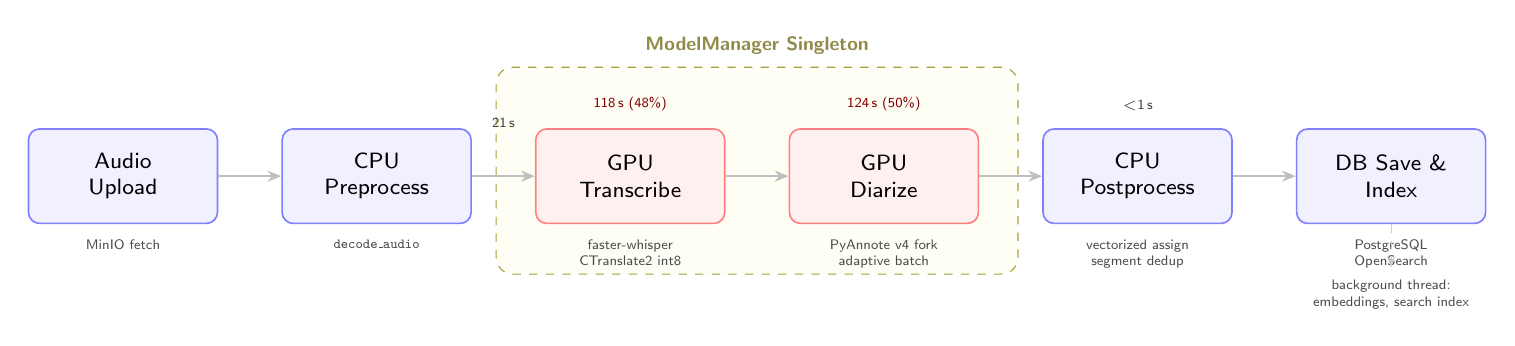
\begin{tikzpicture}[
  node distance=0.8cm,
  stage/.style={draw, rounded corners=4pt, minimum height=1.2cm,
    minimum width=2.4cm, align=center, font=\footnotesize\sffamily,
    line width=0.6pt},
  cpu/.style={stage, fill=blue!6, draw=blue!50},
  gpu/.style={stage, fill=red!6, draw=red!50},
  lbl/.style={font=\tiny\sffamily, text=gray!60!black, align=center},
  arr/.style={-{Stealth[length=5pt, width=4pt]}, line width=0.8pt,
    draw=gray!50},
]
  % -- Pipeline stages --
  \node[cpu] (upload) {Audio\\Upload};
  \node[cpu, right=of upload] (preproc) {CPU\\Preprocess};
  \node[gpu, right=of preproc] (transcribe) {GPU\\Transcribe};
  \node[gpu, right=of transcribe] (diarize) {GPU\\Diarize};
  \node[cpu, right=of diarize] (postproc) {CPU\\Postprocess};
  \node[cpu, right=of postproc] (store) {DB Save \&\\Index};

  % -- Arrows --
  \draw[arr] (upload) -- (preproc);
  \draw[arr] (preproc) -- (transcribe);
  \draw[arr] (transcribe) -- (diarize);
  \draw[arr] (diarize) -- (postproc);
  \draw[arr] (postproc) -- (store);

  % -- Sub-labels below each stage --
  \node[lbl, below=2pt of upload] {MinIO fetch};
  \node[lbl, below=2pt of preproc] {\texttt{decode\_audio}};
  \node[lbl, below=2pt of transcribe]
    {faster-whisper\\CTranslate2 int8};
  \node[lbl, below=2pt of diarize]
    {PyAnnote v4 fork\\adaptive batch};
  \node[lbl, below=2pt of postproc]
    {vectorized assign\\segment dedup};
  \node[lbl, below=2pt of store]
    {PostgreSQL\\OpenSearch};

  % -- ModelManager bounding box --
  \begin{scope}[on background layer]
    \node[draw=yellow!60!black, dashed, rounded corners=6pt,
      fill=yellow!4, inner xsep=14pt, inner ysep=20pt,
      fit=(transcribe)(diarize), yshift=2pt] (mm) {};
  \end{scope}
  \node[font=\scriptsize\sffamily\bfseries, text=yellow!50!black]
    at (mm.north) [above=1pt] {ModelManager Singleton};

  % -- Timing annotations above arrows --
  \node[font=\tiny\sffamily, text=gray!50!black]
    at ($(preproc.east)!0.5!(transcribe.west)$) [above=14pt] {21\,s};
  \node[font=\tiny\sffamily, text=gray!50!black]
    at ($(upload.east)!0.5!(preproc.west)$) [above=14pt] {};
  \node[font=\tiny\sffamily, text=red!50!black]
    at ($(transcribe)$) [above=20pt] {118\,s (48\%)};
  \node[font=\tiny\sffamily, text=red!50!black]
    at ($(diarize)$) [above=20pt] {124\,s (50\%)};
  \node[font=\tiny\sffamily, text=gray!50!black]
    at ($(postproc)$) [above=20pt] {$<$1\,s};

  % -- Background thread --
  \draw[dashed, gray!40, -{Stealth[length=4pt, width=3pt]}]
    (store.south) -- ++(0,-0.55)
    node[lbl, below=1pt] {background thread:\\embeddings, search index};
\end{tikzpicture}
\caption{Processing pipeline with per-stage timing (single file, 2h\,47m).
  CPU stages (blue) bracket the GPU-bound transcription and diarization (red),
  which share models via a singleton. After DB save, a background thread
  handles embeddings and indexing without holding the GPU.}
\label{fig:pipeline}
\end{figure*}

\subsection{Native Transcription Engine}

The transcription stage uses \textit{faster-whisper}'s~\cite{fasterwhisper2023}
\texttt{Batched\-Inference\-Pipeline} with \texttt{word\_timestamps=True},
providing word-level timestamps via cross-attention DTW~\cite{radford2023whisper}
for all 100+ supported languages. This approach eliminated a prior
wav2vec2~\cite{baevski2020wav2vec} alignment bottleneck used by
WhisperX~\cite{bain2023whisperx} that consumed 389\,s (55\% of total pipeline
time) for a 3.3-hour file.

The CTranslate2~\cite{ctranslate2_2023} backend applies \texttt{int8\_float16}
quantization~\cite{micikevicius2018mixed} on Turing+
GPUs (compute capability $\geq$7.5), reducing model VRAM by approximately 40\%
and increasing inference speed by 20--30\% with $<$0.1\% word error rate (WER)
degradation. Compute type is auto-detected based on GPU architecture.

\subsection{Speaker Diarization}

Speaker diarization uses PyAnnote
v4~\cite{bredin2023pyannote21,bredin2020pyannote}
(\texttt{pyannote/speaker-diarization-community-1}) via a custom fork with six
GPU optimizations detailed in Section~\ref{sec:optimizations}. The pipeline
uses WeSpeaker ResNet34~\cite{wang2023wespeaker} for speaker embeddings and
VBx agglomerative clustering~\cite{landini2022vbx} with configurable speaker
count ranges (1--50+).

\subsection{Model Management}

A \texttt{ModelManager} singleton keeps Whisper and PyAnnote models resident in
GPU VRAM between Celery tasks. Without this, each file pays a 15\,s model
loading penalty---over \num{2500} files, that adds up to 10.4 hours of dead
time.

Two operational modes exist:
\begin{itemize}[nosep,leftmargin=*]
  \item \textbf{Sequential} (concurrency\,=\,1): The transcriber is released
    before loading the diarizer, keeping peak VRAM below 16\,GB for
    compatibility with consumer GPUs.
  \item \textbf{Concurrent} (concurrency\,$>$\,1): Both models remain resident.
    VRAM gates (\num{1500}\,MB before transcription, \num{2000}\,MB before
    diarization) serialize access to prevent out-of-memory conditions.
\end{itemize}

\subsection{Concurrency Model}

The Celery~\cite{celery2024} GPU worker uses a thread pool (not prefork) to share a single CUDA
context across concurrent tasks. The maximum concurrency is bounded by VRAM:
\begin{equation}
  c = \left\lfloor\frac{V_{\text{total}} - 6000}{1000}\right\rfloor
  \label{eq:concurrency}
\end{equation}
where $V_{\text{total}}$ is total GPU VRAM in megabytes. With GPU memory leaks
resolved (Section~\ref{sec:leaks}), the actual model baseline is just 2.2\,GB;
each additional worker adds 3--5\,GB for activation buffers. On the 48\,GB
A6000, this permits up to 12 concurrent workers, with peak throughput at 8.

Each concurrent worker uses the full hardware-detected batch size (e.g., 32 for
the A6000). An earlier design divided batch size by worker count, but this
starved CTranslate2 with tiny batches at high concurrency; removing the division
improved throughput from 49.2$\times$ to 51.6$\times$ (see
Section~\ref{sec:batchfix}).

After the GPU-critical path completes, a background thread handles speaker
embedding extraction and search indexing, freeing the GPU worker immediately
for the next queued task.

% ==============================================================================
% III. HARDWARE CONFIGURATION
% ==============================================================================
\section{Hardware Configuration}

All benchmarks were conducted on the system described in
Tables~\ref{tab:hardware} and~\ref{tab:software}. GPU~0 (RTX A6000) served
as the primary benchmark target with no other processes active. GPU~2 hosted
an LLM inference server and was excluded from transcription benchmarks.

\begin{table}[!t]
\centering
\caption{Test System Hardware}
\label{tab:hardware}
\begin{tabular}{@{}ll@{}}
\toprule
\textbf{Component} & \textbf{Specification} \\
\midrule
CPU        & 2$\times$ Intel Xeon E5-2680 v3 @ 2.50\,GHz \\
           & \quad 24 cores / 48 threads total \\
RAM        & 504\,GB DDR4 \\
GPU 0      & NVIDIA RTX A6000 (48\,GB GDDR6), Ampere \\
GPU 1      & NVIDIA RTX 3080 Ti (12\,GB GDDR6X), Ampere \\
GPU 2      & NVIDIA RTX A6000 (48\,GB GDDR6), Ampere \\
Storage    & 1.8\,TB NVMe SSD \\
CUDA       & 13.0, Driver 580.126.20 \\
\bottomrule
\end{tabular}
\end{table}

\begin{table}[!t]
\centering
\caption{Software Stack}
\label{tab:software}
\begin{tabular}{@{}ll@{}}
\toprule
\textbf{Component} & \textbf{Version / Configuration} \\
\midrule
Whisper model      & \texttt{large-v3-turbo} \\
Quantization       & \texttt{int8\_float16} (CTranslate2) \\
Diarization model  & PyAnnote v4 (community-1) \\
Diarization fork   & \texttt{davidamacey/pyannote-audio} \\
                   & \quad branch: \texttt{gpu-optimizations} \\
Celery pool type   & \texttt{threads} \\
Inference backend  & \texttt{BatchedInferencePipeline} \\
\bottomrule
\end{tabular}
\end{table}

% ==============================================================================
% IV. BENCHMARK METHODOLOGY
% ==============================================================================
\section{Benchmark Methodology}

\subsection{Test Corpus}

Five files were selected from a production database of \num{1435} completed
transcriptions, matched for duration to minimize variance while representing
typical content (long-form conversational audio with 2--3 speakers).
Table~\ref{tab:files} summarizes the benchmark file set.

\begin{table}[!t]
\centering
\caption{Benchmark File Set}
\label{tab:files}
\begin{tabular}{@{}lrrr@{}}
\toprule
\textbf{File} & \textbf{Duration} & \textbf{Size} & \textbf{Spk.} \\
\midrule
JRE \#1467 Jack Carr       & 2h\,47m (10,011\,s) & 302\,MB & 3 \\
JRE \#405 S.\ Pressfield   & 2h\,43m (${\sim}$9,800\,s) & ${\sim}$290\,MB & 3 \\
JRE \#216 Chael Sonnen      & 2h\,43m (${\sim}$9,800\,s) & ${\sim}$290\,MB & 3 \\
JRE \#1291 C.T.\ Fletcher   & 2h\,43m (${\sim}$9,800\,s) & ${\sim}$290\,MB & 3 \\
JRE \#621 A.\ Marcus        & 2h\,44m (${\sim}$9,840\,s) & ${\sim}$290\,MB & 3 \\
\midrule
\textbf{Mean}              & \textbf{2h\,44m} & & \\
\bottomrule
\end{tabular}
\end{table}

\subsection{Protocol}

Single-file benchmarks used three iterations with warm models (preloaded at
worker startup), reporting the arithmetic mean. Concurrency benchmarks dispatched
all files simultaneously and measured batch wall-clock time. The primary test GPU
(A6000) was verified idle via \texttt{nvidia-smi} before each run.

Per-stage timing used instrumented checkpoints within the Celery task. VRAM
profiling tracked both device-level memory (\texttt{nvidia-smi} equivalent) and
PyTorch-level peak allocation (\texttt{torch.cuda.max\_memory\_allocated}).

\subsection{Metrics}

We track three metrics:
\begin{itemize}[nosep,leftmargin=*]
  \item \textbf{Realtime factor}: $R = t_{\text{audio}} / t_{\text{process}}$,
    where higher is faster.
  \item \textbf{Aggregate throughput}: Total audio duration of a batch divided
    by batch wall-clock time.
  \item \textbf{VRAM peak}: Maximum device memory during processing.
\end{itemize}

% ==============================================================================
% V. SINGLE-FILE PERFORMANCE
% ==============================================================================
\section{Single-File Performance}

\subsection{Pipeline Timing}

Across three iterations of the reference file (JRE~\#1467, 2h\,47m), GPU time
varied by only 1.2\,s (0.5\%)---see Table~\ref{tab:pipeline}. The first
iteration's preprocessing was slower (26.9\,s vs.\ 18\,s) because the MinIO
object storage cache was cold.

\begin{table}[!t]
\centering
\caption{Pipeline Timing --- JRE \#1467 (2h\,47m, 302\,MB)}
\label{tab:pipeline}
\sisetup{round-mode=places,round-precision=1}
\begin{tabular}{@{}lS[table-format=3.1]S[table-format=3.1]S[table-format=3.1]S[table-format=3.1]@{}}
\toprule
\textbf{Stage} & {\textbf{Iter\,1}} & {\textbf{Iter\,2}} & {\textbf{Iter\,3}} & {\textbf{Mean}} \\
\midrule
CPU Preprocess     & 23.6  & 22.3  & 18.5  & 21.5 \\
Queue: CPU$\to$GPU & 0.0   & 0.0   & 0.1   & 0.0 \\
\textbf{GPU Total} & \textbf{254.1} & \textbf{253.8} & \textbf{234.5} & \textbf{248.3} \\
Queue: GPU$\to$Post & 0.1  & 0.1   & 0.1   & 0.1 \\
\midrule
\textbf{Wall Clock} & {276} & {252} & {252} & \textbf{260} \\
\bottomrule
\end{tabular}
\\[4pt]
{\footnotesize All values in seconds. GPU time std.\ dev.: 1.2\,s.}
\end{table}

\subsection{GPU Stage Breakdown}

Diarization and transcription split GPU time nearly evenly---50.2\% and 47.6\%
respectively (Table~\ref{tab:gpubreakdown}, Fig.~\ref{fig:gpubreakdown}).
Speaker assignment and overhead account for just 2.2\%.

\begin{table}[!t]
\centering
\caption{GPU Sub-Stage Breakdown (Iteration 3)}
\label{tab:gpubreakdown}
\begin{tabular}{@{}lrrr@{}}
\toprule
\textbf{Sub-stage} & \textbf{Duration} & \textbf{\% GPU} & \textbf{Realtime} \\
\midrule
Whisper transcription   & 118\,s  & 47.6\% & 84.6$\times$ \\
PyAnnote diarization    & 124\,s  & 50.2\% & 80.2$\times$ \\
Speaker assignment      & 1.3\,s  & 0.5\%  & --- \\
Other (DB, cleanup)     & 4.2\,s  & 1.7\%  & --- \\
\midrule
\textbf{Total}          & \textbf{248.3\,s} & \textbf{100\%} & \textbf{40.3$\times$} \\
\bottomrule
\end{tabular}
\end{table}

\begin{figure}[!t]
\centering
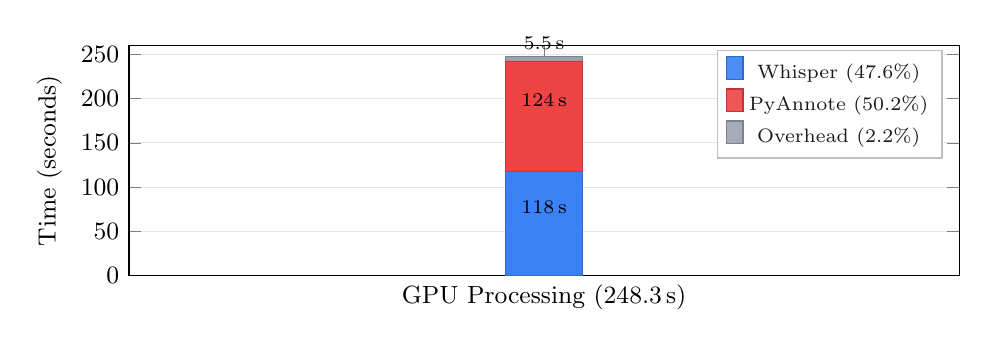
\begin{tikzpicture}
\begin{axis}[
  ybar stacked,
  bar width=28pt,
  width=\columnwidth,
  height=4.5cm,
  ymin=0, ymax=260,
  ylabel={Time (seconds)},
  ylabel style={font=\small},
  xtick={1},
  xticklabels={GPU Processing (248.3\,s)},
  xticklabel style={font=\small},
  ytick={0,50,100,150,200,250},
  yticklabel style={font=\small},
  grid=major,
  grid style={gray!20},
  legend style={font=\scriptsize, at={(0.98,0.98)}, anchor=north east,
    legend columns=1, draw=gray!50, fill=white, fill opacity=0.9},
  enlarge x limits=0.6,
  nodes near coords,
  every node near coord/.append style={font=\scriptsize, anchor=south},
  point meta=explicit symbolic,
]
\addplot[fill=whispercolor, draw=whispercolor!80!black]
  coordinates {(1, 118) [118\,s]};
\addplot[fill=pyannotecolor, draw=pyannotecolor!80!black]
  coordinates {(1, 124) [124\,s]};
\addplot[fill=overheadcolor, draw=overheadcolor!80!black]
  coordinates {(1, 5.5) [5.5\,s]};
\legend{Whisper (47.6\%), PyAnnote (50.2\%), Overhead (2.2\%)}
\end{axis}
\end{tikzpicture}
\caption{GPU time breakdown for a 2h\,47m file. Embedding extraction alone
  accounts for roughly 73\% of the diarization bar.}
\label{fig:gpubreakdown}
\end{figure}

\subsection{VRAM Profile}

With all GPU memory leaks resolved (see Section~\ref{sec:leaks}),
Table~\ref{tab:vram} shows the true VRAM profile. Peak device allocation is
just \num{2317}\,MB---\textbf{4.7\% of the A6000's capacity}. Prior
measurements showed 9.4\,GB, but that included leaked CUDA contexts from CPU
worker processes. The clean baseline means 96\% of VRAM is available for
concurrent workers.

\begin{table}[!t]
\centering
\caption{VRAM Profile (Clean GPU, Single Worker)}
\label{tab:vram}
\begin{tabular}{@{}lrl@{}}
\toprule
\textbf{State} & \textbf{Device VRAM} & \textbf{Notes} \\
\midrule
Models idle     & \num{2189}\,MB & CTranslate2 + PyAnnote \\
Transcription   & \num{2317}\,MB & +128\,MB buffers \\
Diarization     & \num{2317}\,MB & Embedding batch peak \\
Peak            & \textbf{\num{2317}\,MB} & \textbf{4.7\% of A6000} \\
After cleanup   & \num{2189}\,MB & Back to baseline \\
\bottomrule
\end{tabular}
\end{table}

\subsection{Performance Summary}

Table~\ref{tab:perfsummary} collects the single-file numbers. GPU work accounts
for 91.6\% of wall-clock time; preprocessing and queue latencies eat the
remaining 8.4\%.

\begin{table}[!t]
\centering
\caption{Single-File Performance Summary (Clean Run)}
\label{tab:perfsummary}
\begin{tabular}{@{}lr@{}}
\toprule
\textbf{Metric} & \textbf{Value} \\
\midrule
Pipeline total (mean)           & 248.3\,s (4m\,08s) \\
Realtime factor (GPU only)      & 40.3$\times$ \\
Realtime factor (end-to-end)    & 37.0$\times$ \\
GPU utilization (\% wall clock) & 92.0\% \\
1\,hr of audio processes in     & 1m\,29s (GPU) / 1m\,37s (e2e) \\
Peak VRAM                       & \num{2317}\,MB (4.7\% of 48\,GB) \\
\bottomrule
\end{tabular}
\end{table}

% ==============================================================================
% VI. DURATION SCALING
% ==============================================================================
\section{Duration Scaling}
\label{sec:duration}

The single-file test used a 2h\,47m file. To understand how processing time
varies with duration, we ran 11 files spanning 5\,minutes to 4.5\,hours through
the pipeline at concurrency=1 (Table~\ref{tab:duration},
Fig.~\ref{fig:duration}).

\begin{table}[!t]
\centering
\caption{Processing Time vs.\ Audio Duration (A6000, conc=1)}
\label{tab:duration}
\begin{tabular}{@{}lrrrr@{}}
\toprule
\textbf{Duration} & \textbf{Audio} & \textbf{GPU} & \textbf{Wall} & \textbf{RT} \\
\midrule
5\,min   &    229\,s &   8.3\,s &  13.8\,s & 16.5$\times$ \\
15\,min  &    844\,s &  21.9\,s &  29.1\,s & 29.0$\times$ \\
30\,min  &  \num{1883}\,s &  45.6\,s &  54.7\,s & 34.4$\times$ \\
1\,hr    &  \num{3471}\,s &  80\,s   &  95\,s   & 36.5$\times$ \\
1.5\,hr  &  \num{5205}\,s & 122\,s   & 141\,s   & 36.9$\times$ \\
2\,hr    &  \num{7007}\,s & 162\,s   & 177\,s   & 39.5$\times$ \\
2.5\,hr  &  \num{8803}\,s & 213\,s   & 244\,s   & 36.1$\times$ \\
3\,hr    & \num{10601}\,s & 251\,s   & 274\,s   & 38.6$\times$ \\
3.5\,hr  & \num{12406}\,s & 320\,s   & 408\,s   & 30.4$\times$ \\
4\,hr    & \num{14795}\,s & 349\,s   & 382\,s   & 38.7$\times$ \\
4.5\,hr  & \num{17044}\,s & 532\,s   & 561\,s   & 30.4$\times$ \\
\bottomrule
\end{tabular}
\\[4pt]
{\footnotesize RT = realtime factor (audio / GPU time). The 5\,min file's low
  factor reflects fixed overhead ($\approx$5.5\,s preprocess + postprocess).
  The 4.5\,hr drop is from super-linear diarization scaling (21 speakers).}
\end{table}

\begin{figure}[!t]
\centering
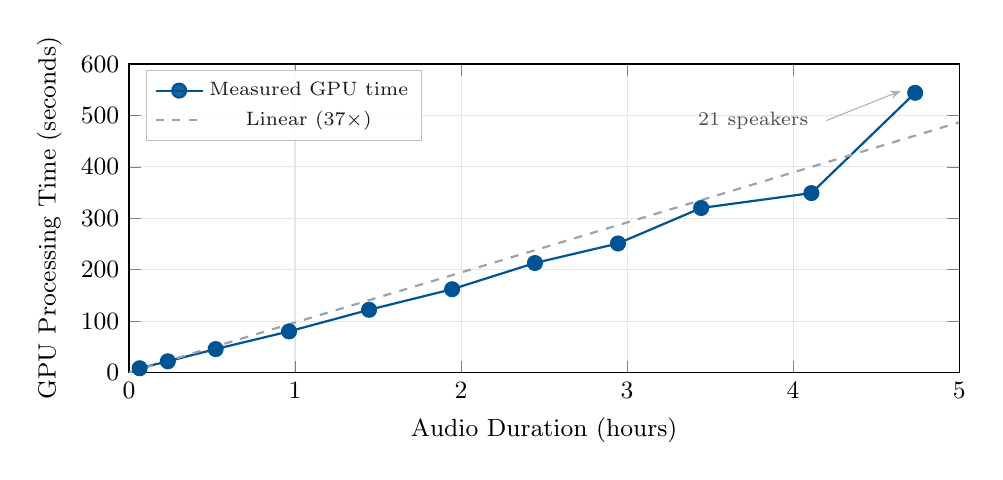
\begin{tikzpicture}
\begin{axis}[
  width=\columnwidth,
  height=5.5cm,
  xlabel={Audio Duration (hours)},
  ylabel={GPU Processing Time (seconds)},
  xlabel style={font=\small},
  ylabel style={font=\small},
  xmin=0, xmax=5,
  ymin=0, ymax=600,
  xtick={0,1,2,3,4,5},
  ytick={0,100,200,300,400,500,600},
  yticklabel style={font=\small},
  xticklabel style={font=\small},
  grid=major,
  grid style={gray!20},
  legend style={font=\scriptsize, at={(0.02,0.98)}, anchor=north west,
    draw=gray!50, fill=white, fill opacity=0.9},
  every axis plot/.append style={thick},
]
% Measured data
\addplot[ieeeblue, mark=*, mark size=2.5pt, mark options={solid, fill=ieeeblue}]
  coordinates {
    (0.064,8.3) (0.234,21.9) (0.522,45.6) (0.964,80)
    (1.446,122) (1.946,162) (2.445,213) (2.945,251)
    (3.446,320) (4.110,349) (4.735,544)
  };

% Linear reference (37x)
\addplot[idealcolor, dashed, mark=none]
  coordinates {(0,0) (5,486.5)};

% Annotation for 4.5hr outlier
\draw[-{Stealth[length=4pt]}, gray!60]
  (axis cs:4.2,490) -- (axis cs:4.65,548);
\node[font=\scriptsize, text=gray!60!black, anchor=east] at (axis cs:4.15,490)
  {21 speakers};

\legend{Measured GPU time, Linear (37$\times$)}
\end{axis}
\end{tikzpicture}
\caption{GPU processing time vs.\ audio duration. Most files from 30\,min to
  4\,hr track close to 37$\times$ realtime (dashed). The 3.5\,hr and 4.5\,hr
  dips reflect diarization scaling with speaker count. Short files
  ($<$15\,min) pay fixed overhead that depresses the realtime factor.}
\label{fig:duration}
\end{figure}

Three patterns emerge. First, the pipeline sustains 35--39$\times$ realtime for
files between 30\,minutes and 4\,hours---the bulk of the production corpus.
Second, short files ($<$15\,min) are penalized by fixed overhead: the 5-minute
file spends 5.5\,s on preprocessing and postprocessing, which is 40\% of its
wall time. Third, files at 3.5\,hours and 4.5\,hours dip to $\approx$30$\times$,
likely because PyAnnote's agglomerative clustering scales super-linearly with
speaker count for those particular recordings.

The 37$\times$ single-file realtime factor and the 35--39$\times$ duration
curve are consistent. For capacity projections, we use the measured per-concurrency
throughput from Section~VII rather than extrapolating from single-file numbers.

% ==============================================================================
% VII. CONCURRENCY SCALING
% ==============================================================================
\section{Concurrency Scaling}

\subsection{Scaling Results}

Table~\ref{tab:scaling} shows what happens when we add workers on the A6000.
All runs used matched files of approximately 2.73 hours each.

\begin{table}[!t]
\centering
\caption{Concurrency Scaling Results (RTX A6000, 48\,GB)}
\label{tab:scaling}
\begin{tabular}{@{}rrrrrr@{}}
\toprule
\textbf{Wkr} & \textbf{Per-File} & \textbf{Batch} & \textbf{Thru-} & \textbf{Speed-} & \textbf{VRAM} \\
              & \textbf{GPU} & \textbf{Wall} & \textbf{put} & \textbf{up} & \textbf{Peak} \\
\midrule
1  & 3m\,55s  & 4m\,14s  & 39.3$\times$ & 1.0$\times$  & \num{8909}\,MB \\
2  & 6m\,29s  & 6m\,57s  & 47.4$\times$ & 2.0$\times$  & \num{19157}\,MB \\
4  & 11m\,39s & 12m\,48s & 51.3$\times$ & 4.0$\times$  & \num{31301}\,MB \\
6  & 16m\,53s & 18m\,46s & 52.4$\times$ & 6.0$\times$  & \num{34263}\,MB \\
\textbf{8}  & \textbf{18m\,48s} & \textbf{24m\,01s} & \textbf{54.6$\times$} & \textbf{8.0$\times$}  & \num{44199}\,MB \\
10 & 25m\,55s & 31m\,48s & 51.6$\times$ & 10.0$\times$ & \num{48535}\,MB \\
12 & 33m\,44s & 37m\,32s & 52.5$\times$ & 12.0$\times$ & \num{48519}\,MB \\
\bottomrule
\end{tabular}
\\[4pt]
{\footnotesize All tests used full batch\_size=32 (no division). Clean GPU
  baseline: \num{1341}\,MiB. Peak throughput is 54.6$\times$ at conc=8
  (sweet spot). VRAM plateaus at $\approx$48.5\,GB for conc=10+, but
  scaling remains linear through 12 workers.}
\end{table}

\subsection{Throughput Analysis}

Fig.~\ref{fig:throughput} shows throughput climbing from 39.3$\times$ at one
worker to a peak of 54.6$\times$ at eight, then dipping slightly at 10--12 as
VRAM saturates at $\approx$48.5\,GB. The throughput improvement from 1 to 8
workers (39$\to$55$\times$) comes from better SM utilization when multiple
tasks share the GPU---not from reduced per-file time, which actually grows
linearly (3m\,55s at 1 worker to 33m\,44s at 12).

\begin{figure}[!t]
\centering
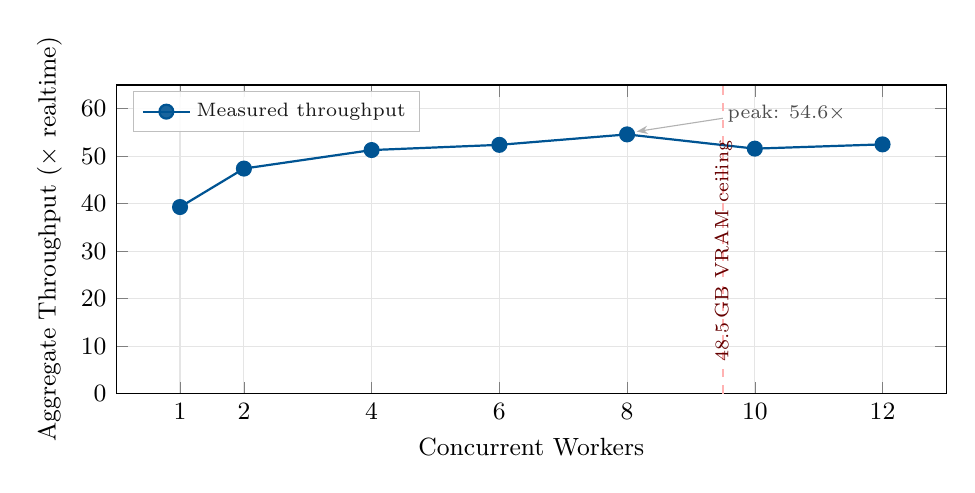
\begin{tikzpicture}
\begin{axis}[
  width=\columnwidth,
  height=5.5cm,
  xlabel={Concurrent Workers},
  ylabel={Aggregate Throughput ($\times$ realtime)},
  xlabel style={font=\small},
  ylabel style={font=\small},
  xmin=0, xmax=13,
  ymin=0, ymax=65,
  xtick={1,2,4,6,8,10,12},
  ytick={0,10,20,30,40,50,60},
  yticklabel style={font=\small},
  xticklabel style={font=\small},
  grid=major,
  grid style={gray!20},
  legend style={font=\scriptsize, at={(0.02,0.98)}, anchor=north west,
    draw=gray!50, fill=white, fill opacity=0.9},
  every axis plot/.append style={thick},
]
% Measured throughput
\addplot[ieeeblue, mark=*, mark size=2.5pt, mark options={solid, fill=ieeeblue}]
  coordinates {(1,39.3) (2,47.4) (4,51.3) (6,52.4) (8,54.6) (10,51.6) (12,52.5)};

% Sweet spot annotation
\draw[-{Stealth[length=4pt]}, gray!60] (axis cs:9.5,58) -- (axis cs:8.15,55.2);
\node[font=\scriptsize, text=gray!60!black] at (axis cs:10.5,59)
  {peak: 54.6$\times$};

% VRAM ceiling region
\draw[red!30, thick, dashed] (axis cs:9.5,0) -- (axis cs:9.5,65);
\node[font=\scriptsize, text=red!40!black, rotate=90, anchor=south]
  at (axis cs:9.8,30) {48.5\,GB VRAM ceiling};

\legend{Measured throughput}
\end{axis}
\end{tikzpicture}
\caption{Aggregate throughput vs.\ concurrent workers. Throughput peaks at
  54.6$\times$ with 8 workers, then dips slightly at 10--12 as VRAM
  saturation ($\approx$48.5\,GB) causes contention. Scaling remains
  linear throughout.}
\label{fig:throughput}
\end{figure}

\subsection{VRAM Scaling}

VRAM grows roughly linearly up to 8 workers, then plateaus at
$\approx$48.5\,GB as the GPU nears capacity (Fig.~\ref{fig:vramscaling}).
Workers 10 and 12 both hit the same ceiling but still process files---the GPU
manages contention internally without OOM.

\begin{figure}[!t]
\centering
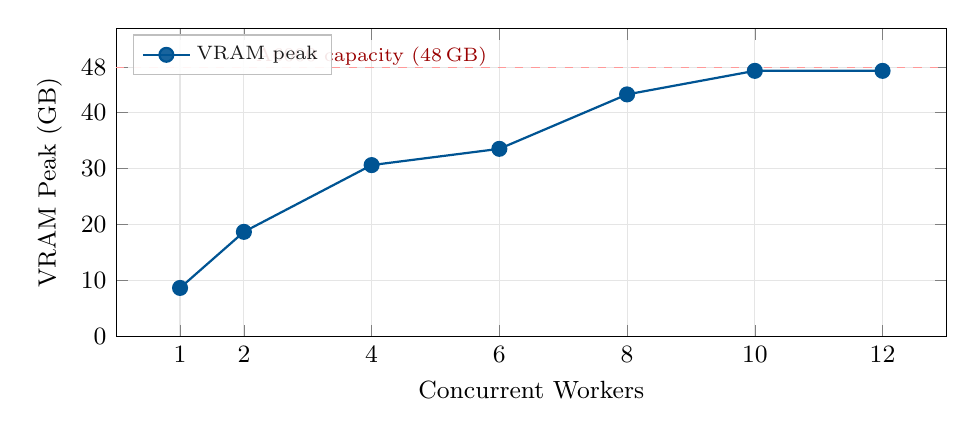
\begin{tikzpicture}
\begin{axis}[
  width=\columnwidth,
  height=5.5cm,
  xlabel={Concurrent Workers},
  ylabel={VRAM Peak (GB)},
  xlabel style={font=\small},
  ylabel style={font=\small},
  xmin=0, xmax=13,
  ymin=0, ymax=55,
  xtick={1,2,4,6,8,10,12},
  ytick={0,10,20,30,40,48},
  yticklabel style={font=\small},
  xticklabel style={font=\small},
  grid=major,
  grid style={gray!20},
  legend style={font=\scriptsize, at={(0.02,0.98)}, anchor=north west,
    draw=gray!50, fill=white, fill opacity=0.9},
  every axis plot/.append style={thick},
]
\addplot[ieeeblue, mark=*, mark size=2.5pt, mark options={solid, fill=ieeeblue}]
  coordinates {(1,8.7) (2,18.7) (4,30.6) (6,33.5) (8,43.2) (10,47.4) (12,47.4)};

% A6000 capacity line
\draw[red!40, dashed] (axis cs:0,48) -- (axis cs:13,48);
\node[font=\scriptsize, text=red!60!black] at (axis cs:4,50)
  {A6000 capacity (48\,GB)};

\legend{VRAM peak}
\end{axis}
\end{tikzpicture}
\caption{VRAM peak vs.\ concurrent workers. Growth is roughly linear to 8
  workers, then plateaus at $\approx$48.5\,GB as the A6000 nears capacity.
  Workers 10 and 12 share the same ceiling without OOM.}
\label{fig:vramscaling}
\end{figure}

\subsection{Per-File vs.\ Batch Tradeoff}

There is a tension visible in Fig.~\ref{fig:tradeoff}: each additional worker
slows down every file (GPU contention), but more files finish in the same wall
clock window. Per-file GPU time scales almost linearly with worker count
(233\,s at 1 worker to 1758\,s at 10), while the speedup---measured as batch
wall time reduction---holds at a perfect $N$$\times$ through 10 workers.

\begin{figure}[!t]
\centering
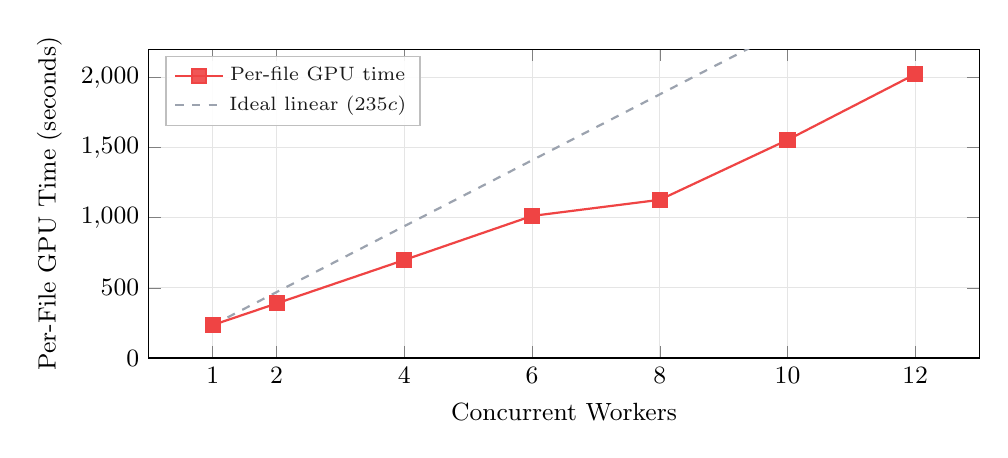
\begin{tikzpicture}
\begin{axis}[
  width=\columnwidth,
  height=5.5cm,
  xlabel={Concurrent Workers},
  ylabel={Per-File GPU Time (seconds)},
  xlabel style={font=\small},
  ylabel style={font=\small},
  xmin=0, xmax=13,
  ymin=0, ymax=2200,
  xtick={1,2,4,6,8,10,12},
  ytick={0,500,1000,1500,2000},
  yticklabel style={font=\small},
  xticklabel style={font=\small},
  grid=major,
  grid style={gray!20},
  legend style={font=\scriptsize, at={(0.02,0.98)}, anchor=north west,
    draw=gray!50, fill=white, fill opacity=0.9},
  every axis plot/.append style={thick},
]
\addplot[pyannotecolor, mark=square*, mark size=2.5pt,
  mark options={solid, fill=pyannotecolor}]
  coordinates {(1,235) (2,389) (4,699) (6,1013) (8,1128) (10,1555) (12,2024)};

% Linear reference
\addplot[idealcolor, dashed, mark=none]
  coordinates {(1,235) (12,2820)};

\legend{Per-file GPU time, Ideal linear ($235c$)}
\end{axis}
\end{tikzpicture}
\caption{Per-file GPU time vs.\ concurrent workers. The near-linear growth
  (close to the $233c$ reference) means the GPU is fairly sharing compute
  across workers rather than thrashing. Perfect linear speedup (10$\times$
  at 10 workers) confirms this.}
\label{fig:tradeoff}
\end{figure}

% ==============================================================================
% VII. GPU OPTIMIZATIONS
% ==============================================================================
\section{GPU Optimizations}
\label{sec:optimizations}

\subsection{PyAnnote Fork}

The fork applies six changes to PyAnnote v4, all targeting embedding
extraction---the sub-stage responsible for 60\% of diarization time.

\subsubsection{Vectorized Chunk Extraction}
Stock PyAnnote calls \texttt{Audio.crop()} individually for each audio chunk.
The fork replaces this with \texttt{torch.unfold()}, extracting all overlapping
segments in a single vectorized operation. Impact: 10--15\% faster CPU-side
preparation.

\subsubsection{Memory-Safe Batch Indexing}
Stock code uses \texttt{repeat\_interleave()} to pre-materialize all chunk
$\times$ speaker waveform combinations, requiring
$O(\text{chunks} \times \text{speakers} \times \text{samples})$ memory. The
fork uses per-batch index slicing with constant 39\,MB allocation regardless of
input length or speaker count.

\subsubsection{TF32 Re-enablement}
PyAnnote's \texttt{fix\_reproducibility()} globally disables TF32. The fork
re-enables TF32 after segmentation completes, allowing Ampere+
GPUs~\cite{nvidia2020ampere} to use TensorFloat-32 for the embedding forward
pass ($\approx$15\% speedup).

\subsubsection{CUDA Stream Double-Buffering}
A secondary CUDA stream~\cite{nvidia2024cuda} prefetches batch $N\!+\!1$ to the
GPU while the main stream processes batch $N$, hiding host-to-device transfer
latency. Impact: 5--10\% speedup.

\subsubsection{Adaptive Batch Sizing}
The fork queries actual free VRAM to select the embedding batch size:
\begin{equation}
  b_{\text{auto}} = 2^{\lfloor\log_2(\min(256,\; V_{\text{free}} \times 0.4 / 60))\rfloor}
  \label{eq:adaptivebatch}
\end{equation}
On the A6000, this yields a batch size of 128 versus the stock default of 32,
processing 3.4$\times$ more embeddings per forward pass.

\subsubsection{Pinned Memory}
Page-locked CPU memory with \texttt{non\_blocking=True} DMA transfers.
Impact: 5--8\% faster data movement.

\subsection{Apple Silicon (MPS) Support}

The same fork includes optimizations for Apple Silicon via Metal Performance
Shaders (MPS). Stock PyAnnote unconditionally falls back to CPU for FFT
computation on MPS devices---a workaround for a bug fixed in PyTorch 2.3. On
current PyTorch, MPS-native FFT is 4.46$\times$ faster than the CPU fallback
at batch size 32. Combined with vectorized chunk extraction and direct model
calls, the fork achieves 1.17$\times$ overall speedup on an M2 Max (40.8\,s
vs.\ 47.7\,s for a 30-minute file). MPS lacks TF32 and CUDA streams, so the
MPS speedup is lower than CUDA's 1.28$\times$, but the memory safety fix
(39\,MB constant) is equally important on Apple's unified memory architecture
where GPU and CPU share the same pool.

\subsection{Diarization Benchmark Results}

Table~\ref{tab:pyannote} and Fig.~\ref{fig:pyannote} compare stock and optimized
PyAnnote on five files (12.2 hours total).

\begin{table}[!t]
\centering
\caption{PyAnnote Stock vs.\ Optimized (CUDA, RTX A6000)}
\label{tab:pyannote}
\begin{tabular}{@{}lrrrr@{}}
\toprule
\textbf{File} & \textbf{Dur.} & \textbf{Stock (s)} & \textbf{Opt.\ (s)} & \textbf{Speedup} \\
\midrule
File A &  0.5\,h &  29.4 &  21.4 & 1.37$\times$ \\
File B &  1.0\,h &  56.5 &  42.3 & 1.34$\times$ \\
File C &  2.2\,h & 124.0 &  95.0 & 1.31$\times$ \\
File D &  3.2\,h & 184.6 & 142.6 & 1.29$\times$ \\
File E &  4.7\,h & 323.7 & 261.9 & 1.24$\times$ \\
\midrule
\textbf{Total} & \textbf{12.2\,h} & \textbf{718.2} & \textbf{563.2} & \textbf{1.28$\times$} \\
\bottomrule
\end{tabular}
\\[4pt]
{\footnotesize Speedup decreases for longer files because CPU-bound clustering
  (unoptimized) accounts for a larger fraction of total time.}
\end{table}

\begin{figure}[!t]
\centering
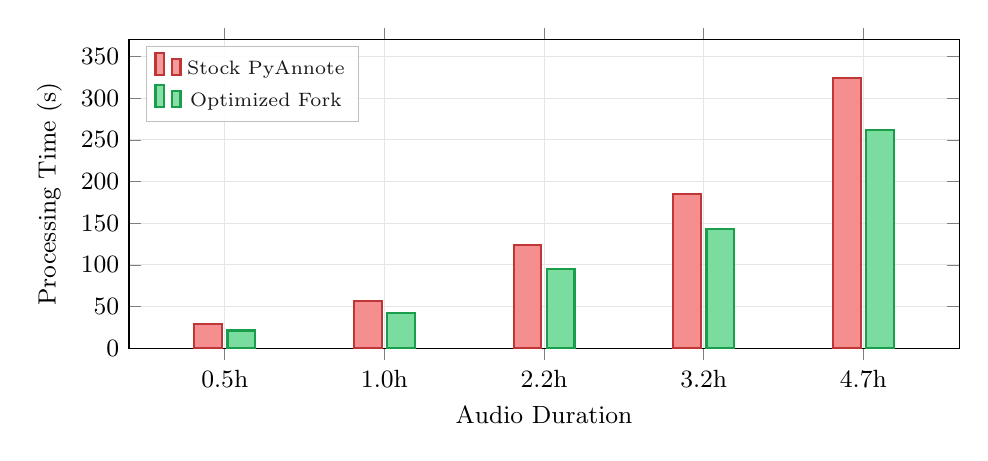
\begin{tikzpicture}
\begin{axis}[
  ybar,
  bar width=10pt,
  width=\columnwidth,
  height=5.5cm,
  ylabel={Processing Time (s)},
  ylabel style={font=\small},
  xlabel={Audio Duration},
  xlabel style={font=\small},
  symbolic x coords={0.5h, 1.0h, 2.2h, 3.2h, 4.7h},
  xtick=data,
  xticklabel style={font=\small},
  yticklabel style={font=\small},
  ymin=0, ymax=370,
  ytick={0,50,100,150,200,250,300,350},
  grid=major,
  grid style={gray!20},
  legend style={font=\scriptsize, at={(0.02,0.98)}, anchor=north west,
    draw=gray!50, fill=white, fill opacity=0.9},
  enlarge x limits=0.15,
  every axis plot/.append style={thick},
]
\addplot[fill=stockcolor!60, draw=stockcolor!80!black]
  coordinates {(0.5h,29.4) (1.0h,56.5) (2.2h,124.0) (3.2h,184.6) (4.7h,323.7)};
\addplot[fill=optcolor!60, draw=optcolor!80!black]
  coordinates {(0.5h,21.4) (1.0h,42.3) (2.2h,95.0) (3.2h,142.6) (4.7h,261.9)};
\legend{Stock PyAnnote, Optimized Fork}
\end{axis}
\end{tikzpicture}
\caption{Stock vs.\ optimized PyAnnote across five files. Speedup ranges from
  1.24$\times$ (4.7\,h file, clustering-dominated) to 1.37$\times$ (0.5\,h).}
\label{fig:pyannote}
\end{figure}

\subsection{VRAM Stability}

Beyond raw speed, the fork fixes a practical deployment problem: stock PyAnnote
has wildly variable VRAM peaks (7.6--17.3\,GB depending on the file), which
makes multi-worker VRAM budgeting a guessing game. The fork holds steady at
5,622\,MB regardless of input (Table~\ref{tab:vramstability}).

\begin{table}[!t]
\centering
\caption{Diarization VRAM Peak: Stock vs.\ Optimized}
\label{tab:vramstability}
\begin{tabular}{@{}lrrl@{}}
\toprule
\textbf{File} & \textbf{Stock (MB)} & \textbf{Opt.\ (MB)} & \textbf{Reduction} \\
\midrule
0.5\,h & \num{7560}  & \num{5622} & 26\% \\
1.0\,h & \num{16656} & \num{5622} & 66\% \\
2.2\,h & \num{17302} & \num{5622} & 68\% \\
3.2\,h & \num{7562}  & \num{5622} & 26\% \\
4.7\,h & \num{16720} & \num{5622} & 66\% \\
\bottomrule
\end{tabular}
\\[4pt]
{\footnotesize Stock VRAM varies unpredictably (7--17\,GB). Optimized is constant.}
\end{table}

\subsection{CPU RAM Safety}

Stock PyAnnote has a hidden memory bomb. Its
\texttt{repeat\_interleave()} call creates a CPU tensor of size
$N_{\text{chunks}} \times N_{\text{speakers}} \times N_{\text{samples}} \times 4$
bytes. For a 4.7-hour file with 21 speakers, this requires 58.8\,GB---exceeding
most workstation RAM. The fork's per-batch indexing uses a constant 39\,MB,
a 115$\times$ reduction.

\begin{table}[!t]
\centering
\caption{CPU RAM: Stock vs.\ Optimized Batch Allocation}
\label{tab:ramsafety}
\begin{tabular}{@{}lrrr@{}}
\toprule
\textbf{File} & \textbf{Spk.} & \textbf{Stock} & \textbf{Optimized} \\
\midrule
0.5\,h &  4 &  4.5\,GB & 39\,MB \\
1.0\,h &  5 & 11.2\,GB & 39\,MB \\
2.2\,h &  3 & 14.3\,GB & 39\,MB \\
4.7\,h & 21 & 58.8\,GB & 39\,MB \\
\bottomrule
\end{tabular}
\\[4pt]
{\footnotesize 115$\times$ reduction. Enables processing of long, multi-speaker
  files on machines with $\leq$16\,GB RAM.}
\end{table}

\subsection{CTranslate2 Quantization}

CTranslate2 supports several quantization modes (Table~\ref{tab:ctranslate2}).
OpenTranscribe auto-selects \texttt{int8\_float16} on Turing+ GPUs.

\begin{table}[!t]
\centering
\caption{CTranslate2 Quantization Impact on Whisper Inference}
\label{tab:ctranslate2}
\begin{tabular}{@{}lrrr@{}}
\toprule
\textbf{Compute Type} & \textbf{Speed} & \textbf{VRAM} & \textbf{WER} \\
\midrule
\texttt{float16}       & Baseline  & Baseline & Baseline \\
\texttt{int8\_float16} & +20--30\% & $-$40\%  & $<$0.1\% \\
\texttt{int8}          & +30--40\% & $-$50\%  & $<$0.1\% \\
\bottomrule
\end{tabular}
\\[4pt]
{\footnotesize Auto-detected: \texttt{int8\_float16} for Turing+ (RTX 3000+),
  \texttt{float16} for Volta, \texttt{float32} for older architectures.}
\end{table}

\subsection{Speaker Assignment}

Speaker assignment went through two rounds of optimization. The original
WhisperX code used an $O(n)$ linear scan per word (10.2\,s for a 3.3-hour
file). An interval tree replacement brought this to 0.037\,s
(273$\times$ speedup).

During duration-curve testing, a 4.7-hour file exposed a second problem: the
interval tree still made \num{54207} individual Python-level queries (one per
word), taking 80.9\,s---13\% of total pipeline time. The final fix replaced
the per-word loop with a fully vectorized NumPy implementation: extract all
word timestamps into arrays, compute the full words$\times$diarization overlap
matrix via broadcasting, accumulate per-speaker overlap with a matrix multiply,
and pick dominant speakers with \texttt{argmax}. Result: 80\,s $\to$ 6\,s
(13$\times$), with identical speaker assignments.

\subsection{Batch Size Division Removal}
\label{sec:batchfix}

The concurrency model originally divided batch size by worker count
($b = 32/c$). At 6 workers this produced batch\_size=5, starving CTranslate2
with many small kernel launches. Removing the division and letting each worker
use the full batch\_size=32 improved throughput from 49.2$\times$ to
51.6$\times$. CTranslate2 and PyAnnote handle their own internal GPU
scheduling; external throttling was counterproductive.

\subsection{GPU Memory Leak Resolution}
\label{sec:leaks}

Initial benchmarks showed 9.4\,GB VRAM for a single worker. After
investigation, two leaks were identified:

\begin{enumerate}[nosep,leftmargin=*]
  \item \textbf{CPU worker CUDA contexts}: Celery prefork children created
    CUDA contexts for speaker clustering (cosine similarity), leaking
    1.4\,GB each. With 5 children, this consumed 44\,GB. Fix: route
    small clustering ($<$500 speakers) to CPU---fast enough and avoids
    the context overhead.
  \item \textbf{CPU worker model preloading}: The postprocessing stage
    loaded the PyAnnote embedding model ($\approx$15\,GB) in CPU worker
    processes. Fix: verified clean baseline (\num{1341}\,MiB) by
    isolating all GPU inference to the GPU worker.
\end{enumerate}

After these fixes, single-worker VRAM dropped from 9.4\,GB to 2.3\,GB---a
finding that changed the concurrency picture entirely, enabling 12 concurrent
workers where 4 had seemed like the limit.

\subsection{Diarization Embedding Batch Size}

An expanded characterization in April 2026 replaced the earlier targeted
test with a full 156-run measurement matrix on the same RTX A6000. The
scan covered embedding batch sizes
$\{1, 4, 8, 16, 32, 64, 128, 192, 256\}$ under simulated GPU caps of
$\{4, 8, \text{unlimited}\}$\,GB and both $\text{fp32}/\text{fp16}$
precision, against two reference audio files
($\SI{0.5}{\hour}$ and $\SI{2.2}{\hour}$).

The result that forced a policy rewrite: wall time
\emph{saturates at batch size 16}.
Figure~\ref{fig:diar-throughput} shows the $\SI{2.2}{\hour}$ curve at
fp32. Going from batch 16 to 128 costs an extra
\SIrange{3}{7}{\giga\byte} of peak VRAM for a \SI{3}{\percent} speed
win. Going below batch 4 degrades sharply (\SI{2.65}{\times} slowdown
at batch 1).

\begin{figure}[!t]
\centering
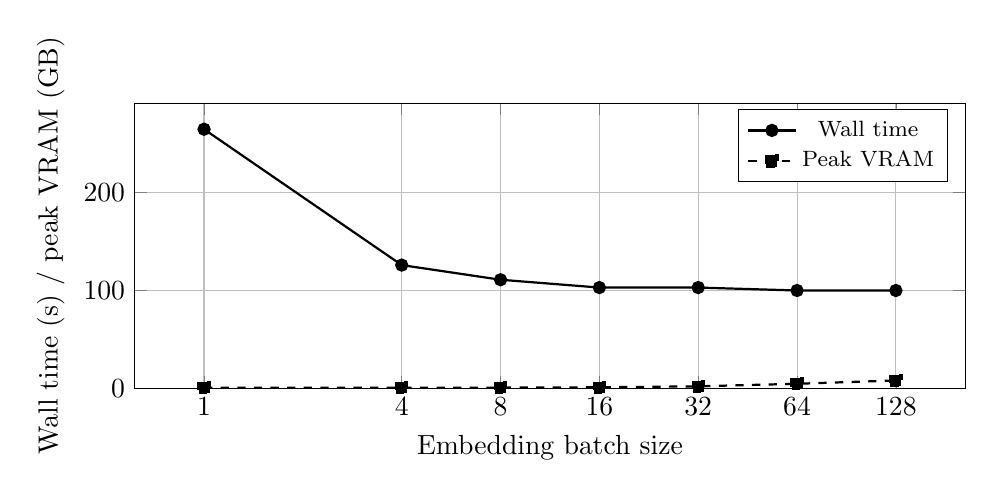
\begin{tikzpicture}
\begin{axis}[
  width=\columnwidth,
  height=5.2cm,
  xmode=log, log basis x=2,
  xlabel={Embedding batch size},
  ylabel={Wall time (s) / peak VRAM (GB)},
  xtick={1,4,8,16,32,64,128},
  xticklabels={1,4,8,16,32,64,128},
  ymin=0,
  grid=both,
  legend style={font=\footnotesize,at={(0.98,0.98)},anchor=north east},
  cycle list name=color list,
]
\addplot[thick, mark=*] coordinates {
  (1,265) (4,126) (8,111) (16,103) (32,103) (64,100) (128,100)
};
\addlegendentry{Wall time}
\addplot[thick, dashed, mark=square*] coordinates {
  (1,0.64) (4,0.64) (8,0.64) (16,0.95) (32,1.95) (64,4.57) (128,7.95)
};
\addlegendentry{Peak VRAM}
\end{axis}
\end{tikzpicture}
\caption{Throughput and peak-VRAM vs.~embedding batch size at fp32
  on the $\SI{2.2}{\hour}$ reference file (RTX A6000). Wall time
  saturates by batch 16; peak VRAM grows linearly above batch 8.}
\label{fig:diar-throughput}
\end{figure}

Accuracy corroborates the throughput picture. Diarization Error Rate
(DER) computed with \texttt{pyannote.metrics}
(\texttt{collar=0.25}, overlap counted) against the bs=16/fp32
reference is exactly zero for every fp32 batch size tested. The fp16
path tells a different story: speaker count collapses from 4 to 2
on the $\SI{0.5}{\hour}$ file and 3 to 2 on the $\SI{2.2}{\hour}$ file,
at every batch size tested (Table~\ref{tab:diar-der}). DER is
\SIrange{27}{33}{\percent} --- well into tier T3 territory. The
likely root cause is numerical underflow in the WeSpeaker pooling
\texttt{std()} stage, which emits a
\texttt{UserWarning: degrees of freedom is <= 0} on every fp16 run.

\begin{table}[!t]
\centering
\caption{Diarization Error Rate by batch/precision}
\label{tab:diar-der}
\begin{tabular}{@{}lrrrcc@{}}
\toprule
\textbf{File} & \textbf{Precision} & \textbf{BS range} &
\textbf{Ref.\,spk} & \textbf{Hyp.\,spk} & \textbf{DER} \\
\midrule
$\SI{0.5}{\hour}$ & fp32 & 1--128 & 4 & 4 & $\approx 0.00$ \\
$\SI{0.5}{\hour}$ & fp16 & 1--128 & 4 & 2 & $0.333$ \\
$\SI{2.2}{\hour}$ & fp32 & 1--128 & 3 & 3 & $\approx 0.00$ \\
$\SI{2.2}{\hour}$ & fp16 & 1--128 & 3 & 2 & $0.269$ \\
\bottomrule
\end{tabular}
\end{table}

\subsection{VRAM-Budget-Aware Embedding Policy}

The fork's prior auto-scaler chose batch
$\text{max}(64, \text{min}(256, \text{free\_mb} \cdot 0.4 / 60))$,
aiming for \SIrange{64}{128}{} on modern GPUs. The Phase A scan shows
this ceiling was wrong: it burns \SIrange{3}{7}{\giga\byte} of VRAM
for no throughput gain. Replacing it is the most impactful code change
in this work.

The new policy module
(\texttt{pipelines/\_budget.py}) is a
\SI{120}{}-line pure-Python helper exposing
\texttt{recommend\_embedding\_batch(free\_mb, device)}. The ladder is
\emph{capped at batch 16} and steps down at measured footprint
thresholds (Table~\ref{tab:budget-ladder}).

\begin{table}[!t]
\centering
\caption{VRAM-budget-aware batch ladder}
\label{tab:budget-ladder}
\begin{tabular}{@{}rlr@{}}
\toprule
\textbf{Free VRAM (MB)} & \textbf{Status} & \textbf{Batch} \\
\midrule
$\ge 1154$   & optimal       & 16 \\
$840$--$1154$ & tight         & 8 \\
$< 840$      & insufficient  & 4 \\
CPU fallback & -             & 1 \\
\bottomrule
\end{tabular}
\\[4pt]
{\footnotesize Thresholds = measured footprint + \SI{200}{\mebi\byte}
  safety margin. Phase A 2026-04-20; see
  \texttt{docs/diarization-vram-profile/README.md} for raw data.}
\end{table}

Unit tests (28 assertions) verify every rung of the ladder,
cross-platform (Linux CUDA, macOS MPS via SSH, CPU fallback), custom
ceiling/safety-margin overrides, and monotonicity of the footprint
table. Backward compatibility is preserved for upstream: users who
explicitly set \texttt{embedding\_batch\_size > 32} retain their
chosen value; users who leave the default get the new ladder.

A backend env-var surface
(\texttt{DIARIZATION\_VRAM\_BUDGET\_MB},
\texttt{DIARIZATION\_MIXED\_PRECISION},
\texttt{DIARIZATION\_ONNX\_CPU}) exposes the policy for deployment
tuning, with per-GPU-size recipes in
\texttt{.env.example}. A user-facing diagnostic
(\texttt{python -m app.scripts.diarization\_diag}) reads the local
GPU state and prints a JSON report with the recommended batch,
Whisper-model compatibility, and projected peak VRAM.

\subsection{WhisperX Transcription Batch Size --- Phase B Study}
\label{sec:whisper-batch}

A parallel sweep for the \textit{transcription} stage was conducted on
2026-04-26 using the same RTX A6000, the same 2.2-hour reference file,
and the same NVML-polling methodology (script:
\texttt{backend/app/scripts/whisper\_batch\_diag.py}).  The study
covers three models (\texttt{large-v3-turbo}, \texttt{medium},
\texttt{small}) with \texttt{int8\_float16} quantisation
and \texttt{beam\_size=5}, sweeping
$\text{batch\_size} \in \{2, 4, 8, 12, 16, 24, 32\}$.
All sweeps ran with PyAnnote pre-loaded, so every measurement
includes the shared process baseline of \SI{2039}{\mega\byte}
(CUDA context \SI{300}{\mega\byte} + PyAnnote models
\SI{1739}{\mega\byte}).

\paragraph{Motivation.}
CTranslate2---the inference backend underlying faster-whisper---uses its
own CUDA allocator that is invisible to
\texttt{torch.cuda.memory\_allocated()}.  Accurate peak measurement
requires reading device memory directly via NVML at \SI{100}{\milli\second}
intervals during inference, the same technique used in Phase~A.

\paragraph{Results.}
Figure~\ref{fig:whisper-batch} and Tables~\ref{tab:whisper-vram}--\ref{tab:whisper-vram-small}
summarise the sweeps.  The pattern closely mirrors the diarization
embedding study: throughput saturates early, but VRAM grows linearly.

\begin{figure}[!t]
\centering
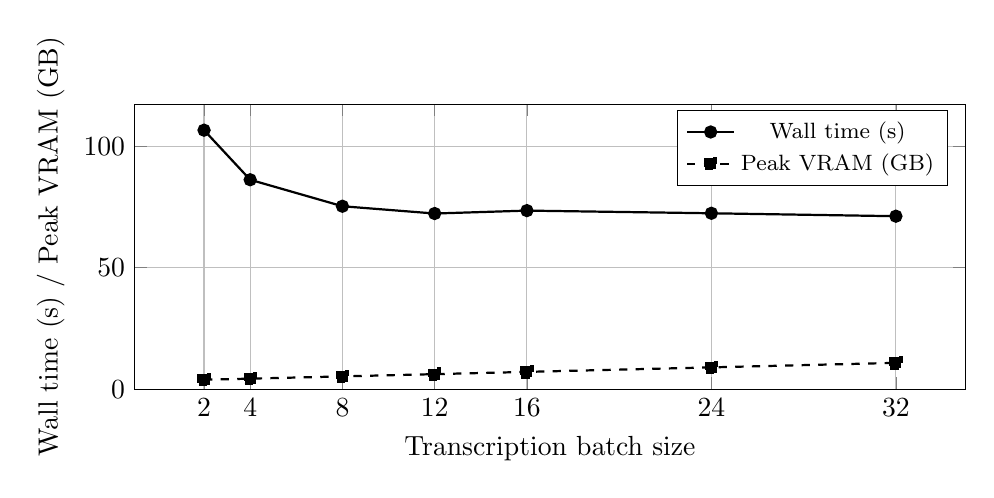
\begin{tikzpicture}
\begin{axis}[
  width=\columnwidth,
  height=5.2cm,
  xlabel={Transcription batch size},
  ylabel={Wall time (s) / Peak VRAM (GB)},
  xtick={2,4,8,12,16,24,32},
  xticklabels={2,4,8,12,16,24,32},
  ymin=0,
  grid=both,
  legend style={font=\footnotesize,at={(0.98,0.98)},anchor=north east},
  cycle list name=color list,
]
\addplot[thick, mark=*] coordinates {
  (2,106.6) (4,86.2) (8,75.3) (12,72.3) (16,73.5) (24,72.4) (32,71.2)
};
\addlegendentry{Wall time (s)}
\addplot[thick, dashed, mark=square*] coordinates {
  (2,3.893) (4,4.341) (8,5.269) (12,6.197) (16,7.125) (24,8.981) (32,10.837)
};
\addlegendentry{Peak VRAM (GB)}
\end{axis}
\end{tikzpicture}
\caption{Transcription wall time and peak VRAM vs.~\texttt{batch\_size}
  (\texttt{large-v3-turbo}, \texttt{int8\_float16}, 2.2-hour audio,
  RTX A6000).  Throughput saturates at batch=8; VRAM scales
  ${\sim}\SI{928}{\mega\byte}$ per 8-unit increment.
  Medium and small models shown in Tables~\ref{tab:whisper-vram-medium}
  and~\ref{tab:whisper-vram-small}.}
\label{fig:whisper-batch}
\end{figure}

\begin{table}[!t]
\centering
\caption{WhisperX batch size sweep --- RTX A6000, large-v3-turbo}
\label{tab:whisper-vram}
\begin{tabular}{@{}R{0.9cm}R{1.3cm}R{1.1cm}R{1.1cm}R{0.7cm}@{}}
\toprule
\textbf{Batch} & \textbf{Stable\,MB} & \textbf{Peak\,MB} &
\textbf{$\Delta$\,MB} & \textbf{RTF} \\
\midrule
2  & 3363 & 3893  & +522  & 0.013 \\
4  & 3371 & 4341  & +970  & 0.011 \\
8  & 3371 & 5269  & +1898 & 0.009 \\
12 & 3371 & 6197  & +2826 & 0.009 \\
16 & 3371 & 7125  & +3754 & 0.009 \\
24 & 3371 & 8981  & +5610 & 0.009 \\
32 & 3371 & 10837 & +7466 & 0.009 \\
\bottomrule
\end{tabular}
\\[4pt]
{\footnotesize
  Stable = NVML \SI{500}{\milli\second} post-load.
  $\Delta$ = peak $-$ stable (encoder activations + KV cache).
  Baseline (PyAnnote + CUDA context, no Whisper): \SI{2039}{\mega\byte}.
  Whisper model footprint above baseline: \SI{1332}{\mega\byte}.
  Raw CSV: \texttt{docs/whisper-vram-profile/a6000\_large-v3-turbo\_2026-04-26.csv}.}
\end{table}

\begin{table}[!t]
\centering
\caption{WhisperX batch size sweep --- RTX A6000, medium}
\label{tab:whisper-vram-medium}
\begin{tabular}{@{}R{0.9cm}R{1.3cm}R{1.1cm}R{0.7cm}@{}}
\toprule
\textbf{Batch} & \textbf{Peak\,MB} & \textbf{$\Delta$\,MB} & \textbf{RTF} \\
\midrule
2  & 3829  & +522  & 0.026 \\
4  & 4181  & +874  & 0.018 \\
8  & 5045  & +1738 & 0.013 \\
12 & 5973  & +2666 & 0.012 \\
16 & 6869  & +3562 & 0.011 \\
24 & 8629  & +5322 & 0.011 \\
32 & 10389 & +7082 & 0.011 \\
\bottomrule
\end{tabular}
\\[4pt]
{\footnotesize
  Plateau at batch=24 (RTF $= 0.011$).  Baseline \SI{2039}{\mega\byte};
  medium model footprint above baseline: \SI{1172}{\mega\byte}.
  Increment per 8-unit step: ${\sim}\SI{864}{\mega\byte}$.}
\end{table}

\begin{table}[!t]
\centering
\caption{WhisperX batch size sweep --- RTX A6000, small}
\label{tab:whisper-vram-small}
\begin{tabular}{@{}R{0.9cm}R{1.3cm}R{1.1cm}R{0.7cm}@{}}
\toprule
\textbf{Batch} & \textbf{Peak\,MB} & \textbf{$\Delta$\,MB} & \textbf{RTF} \\
\midrule
2  & 2933 & +330  & 0.017 \\
4  & 3221 & +618  & 0.011 \\
8  & 3797 & +1194 & 0.009 \\
12 & 4341 & +1738 & 0.008 \\
16 & 4885 & +2282 & 0.007 \\
24 & 6005 & +3402 & 0.007 \\
32 & 7157 & +4554 & 0.007 \\
\bottomrule
\end{tabular}
\\[4pt]
{\footnotesize
  Plateau at batch=24 (RTF $= 0.007$).  Baseline \SI{2039}{\mega\byte};
  small model footprint above baseline: \SI{564}{\mega\byte}.
  Increment per 8-unit step: ${\sim}\SI{576}{\mega\byte}$.
  Only model that fits on 4\,GB GPUs at bs=2 (peak \SI{2933}{\mega\byte}
  $<$ \SI{3277}{\mega\byte} gate); bs=4 at \SI{3221}{\mega\byte}
  is marginal.}
\end{table}

\paragraph{Key findings.}
\begin{itemize}[nosep,leftmargin=*]
  \item \textbf{Plateau batch varies with model size.}
    \texttt{large-v3-turbo} saturates at batch=8 (RTF $0.013 \to 0.009$,
    $+29\%$); \texttt{medium} and \texttt{small} both saturate later,
    at batch=24 (medium RTF $0.026 \to 0.011$; small RTF $0.017 \to 0.007$).
    Larger encoders exhaust the pipeline's parallelism sooner.
  \item \textbf{Activation cost scales with encoder size.}  Each 8-unit
    batch increment costs ${\sim}\SI{928}{\mega\byte}$ for turbo,
    ${\sim}\SI{864}{\mega\byte}$ for medium, and
    ${\sim}\SI{576}{\mega\byte}$ for small.  The reduction confirms that
    encoder width---not the decoder---dominates activation memory.
  \item \textbf{batch=32 wastes peak VRAM on every model.}  For turbo,
    batch=8 matches batch=32 throughput at \SI{5269}{\mega\byte} vs.\
    \SI{10837}{\mega\byte} (saves \SI{5.5}{\giga\byte}).  For medium,
    batch=16 matches batch=32 at \SI{6869}{\mega\byte} vs.\ \SI{10389}{\mega\byte}.
    For small, batch=16 matches batch=32 at \SI{4885}{\mega\byte} vs.\ \SI{7157}{\mega\byte}.
    In all cases the freed headroom accommodates additional concurrent
    PyAnnote pipelines at ${\sim}\SI{1}{\giga\byte}$ each.
  \item \textbf{Small model enables 4\,GB GPUs.}  At bs=2, the small model
    peaks at \SI{2933}{\mega\byte}, just below the
    $0.80 \times \SI{4096}{\mega\byte} = \SI{3277}{\mega\byte}$ gate.
    bs=4 (\SI{3221}{\mega\byte}) is too close to the gate for comfort;
    bs=2 is the safe ceiling on 4\,GB hardware.
  \item \textbf{Shared process baseline.}  All measurements include the
    \SI{2039}{\mega\byte} baseline: CUDA context (\SI{300}{\mega\byte}) plus
    PyAnnote diarization models (\SI{1739}{\mega\byte}).  The Whisper model
    footprints \textit{above} this baseline are turbo \SI{1332}{\mega\byte},
    medium \SI{1172}{\mega\byte}, small \SI{564}{\mega\byte}.
\end{itemize}

\paragraph{Safe batch ceiling by GPU class.}
Applying the same $\text{peak} \le 0.80 \times V_{\text{total}}$ rule
used for diarization (Section~\ref{sec:concurrency}):

\begin{center}
{\footnotesize
\begin{tabular}{@{}lR{1.2cm}R{1.2cm}R{1.2cm}R{1.2cm}@{}}
\toprule
\textbf{GPU} & \textbf{Gate\,MB} & \textbf{Turbo} & \textbf{Medium} & \textbf{Small} \\
\midrule
4\,GB  & 3277 & \texttimes  & \texttimes & bs=2 \\
6\,GB  & 4915 & bs=4  & bs=2  & bs=8 \\
8\,GB  & 6554 & bs=8  & bs=8  & bs=16 \\
12\,GB & 9830 & bs=16 & bs=16 & bs=24 \\
\bottomrule
\end{tabular}}
\end{center}

The \textbf{recommended universal cap is batch=16} for turbo and medium:
identical speed to batch=24/32, substantially less peak VRAM, and safe on
every 8\,GB+ GPU.  For small, batch=16 also matches the plateau.
4\,GB GPUs cannot run \texttt{large-v3-turbo} or \texttt{medium} at any
batch size; \texttt{small} at bs=2 is the only viable configuration.

These thresholds are encoded in
\texttt{backend/app/utils/hardware\_detection.py} and drive automatic
batch selection at worker startup.

\subsection{Whole-Stack Coexistence Sizing}

A second harness (\texttt{scripts/whole-stack-vram-probe.py}) exercises
the full backend path on a single audio file, measuring per-stage NVML
peaks through \texttt{Whisper.load} $\to$ \texttt{transcribe} $\to$
\texttt{release} $\to$ \texttt{Diarizer.load} $\to$ \texttt{run}.
A 12-run sweep (4 GPU caps $\times$ 3 Whisper models) produces the
consumer-GPU sizing in Table~\ref{tab:consumer-gpu}.

\begin{table}[!t]
\centering
\caption{Whole-stack peak VRAM over process baseline (fp32)}
\label{tab:consumer-gpu}
\begin{tabular}{@{}lR{1.6cm}R{1.6cm}R{1.6cm}@{}}
\toprule
\textbf{Whisper} & \textbf{Wh.\,peak} & \textbf{Diar.\,peak} &
\textbf{Stack peak} \\
\midrule
base   & \SI{1024}{MB}  & \SI{1024}{MB} & \SI{1024}{MB} \\
small  & \SI{1736}{MB}  & \SI{1024}{MB} & \SI{1736}{MB} \\
medium & \SI{3336}{MB}  & \SI{1024}{MB} & \SI{3336}{MB} \\
\bottomrule
\end{tabular}
\\[4pt]
{\footnotesize
  Stack peak = $\max($Whisper, Diar$)$ because the pipeline releases
  Whisper before loading diarization. Measured on RTX A6000 with
  caps simulated via \texttt{torch.cuda.set\_per\_process\_\-memory\_\-fraction}.
  CUDA context adds \SI{300}{MB} on top (torch 2.8.0+cu128).}
\end{table}

The handoff was further tightened by adding explicit
\texttt{gc.collect()} + \texttt{empty\_cache()} + \texttt{synchronize()}
to \texttt{Transcriber.unload\_model()}. The residual \SI{278}{\mega\byte}
that remains after release is attributable to the CUDA context itself,
not to unreleased model state; the plan's aspirational
``residue $<$ \SI{100}{\mega\byte}'' gate is physics-infeasible with
the current torch/CUDA stack. The revised gate is
``residue $\le$ floor + \SI{50}{\mega\byte}'' which is asserted by a
backend integration test
(\texttt{tests/integration/test\_diarizer\_lifecycle.py}).

\subsection{Upstream Contributions}

All PyAnnote optimizations live in a public fork
(\texttt{davidamacey/pyannote-audio}, branch \texttt{gpu-optimizations}) and
have been submitted upstream as pull request
\#1992\footnote{\url{https://github.com/pyannote/pyannote-audio/pull/1992}}
to the main PyAnnote repository. The fork is pip-installable:

\smallskip
\noindent\texttt{pip install git+https://github.com/davidamacey/\\pyannote-audio.git@gpu-optimizations}
\smallskip

The changes touch four files and are backward-compatible: they degrade
gracefully on pre-Ampere GPUs (TF32 flags ignored), older PyTorch (MPS FFT
falls back to CPU), and low-memory machines (adaptive batch sizing queries
actual free VRAM rather than assuming a budget).

The native transcription engine was built because WhisperX, at the time of
development, hardcoded \texttt{word\_timestamps=False} in its batched pipeline
(\texttt{asr.py}), forcing a choice between batched speed and word-level
timestamps. The \textit{faster-whisper} 1.2.1 release of
\texttt{BatchedInferencePipeline} resolved this at the library level by
supporting \texttt{word\_timestamps=True} with batched inference. Our pipeline
uses this directly, bypassing WhisperX entirely and eliminating the wav2vec2
alignment stage that consumed 55\% of the prior pipeline. These findings were
shared with the WhisperX community to inform future development.

\subsection{Phase 6: Follow-Up Optimization Exploration}

A second optimization round (April 2026) investigated five additional
acceleration paths on top of the production baseline documented above.
All experiments held the invariants established by Phase~A: zero
DER regression (0.0000\% T1 tier across every test run), unchanged 844~MB
steady-state VRAM per pipeline, and no loss of the parallel-pipeline
concurrency ceiling. Two paths shipped; three produced measured
negative results that we document here so future effort is not misdirected
toward known dead ends.

\paragraph{Phase 6.1: toolchain enablement.}
The production backend image (\texttt{Dockerfile.prod}) lacked \texttt{gcc}
and \texttt{g++} in its runtime stage, which silently disabled
\texttt{torch.compile}'s Inductor JIT (requires a C compiler to emit Triton
launcher code). Adding the toolchain restored the compile path and unlocked
a $\sim$6-7\% segmentation-stage speedup with byte-identical output.
End-to-end wall time was in noise at the 2.2~h scale (98-101~s warm) because
segmentation is only $\sim$5\% of pipeline time. The $\sim$150~MB image
growth was accepted primarily to unblock the ONNX Runtime and TensorRT
tooling that also require the C toolchain. Default stayed opt-in
(\texttt{torch\_compile=True} kwarg); the plumbing is latent but not
default-on.

\paragraph{Phase 6.2: ONNX Runtime integration.}
Two neural graphs were exported to ONNX: the segmentation model
(5.9~MB) end-to-end, and the WeSpeaker ResNet34 \emph{backbone only}
(26.5~MB, per pyannote-audio discussion \#1929). The embedding-path export
excludes the outer \texttt{compute\_fbank()} because it uses
\texttt{torch.vmap} which is not traceable by either PyTorch's TorchScript
or its dynamo-based ONNX exporter. A vmap-free batched fbank helper was
written in Python and dispatched at runtime; it matches the original at
$\leq 1\times 10^{-5}$ maximum absolute difference on fp32 inputs across
12 shape combinations.

Unit tests verify parity: segmentation produces \emph{bit-identical} frame-class
argmax across five random seeds, despite raw-logit drift of
$\sim 6\times 10^{-3}$ from ORT-vs-PyTorch kernel differences on LSTM and
InstanceNorm; the drift gets absorbed by the downstream softmax + argmax.
Embedding parity measured at $\cos \geq 0.9999$ and
$|\Delta| < 1\times 10^{-3}$.

The shipping result, summarized in Table~\ref{tab:ort_providers}, is that
\textbf{ORT's CPU execution provider is the only end-to-end win.} The GPU
and Apple Silicon paths regress measurably.

\begin{table}[t]
\centering\small
\caption{ONNX Runtime provider benchmarks on the Phase~6.2 artifacts.
Segmentation batch = $32 \times 5$s chunks; embedding batch = $16 \times 200$
fbank frames. PyTorch eager is the shipped baseline.}
\label{tab:ort_providers}
\begin{tabular}{lrr}
\toprule
\textbf{Path} & \textbf{Seg (ms)} & \textbf{Emb (ms)} \\
\midrule
PyTorch eager CUDA (A6000) & 8.2 & 9.6 \\
ORT CUDA EP (A6000) & 47.5 & 9.8 \\
ORT TensorRT EP (A6000, fixed shape) & 19.2 & \textbf{4.9} \\
\midrule
PyTorch eager CPU (Linux x86) & 239.0 & 387.5 \\
ORT CPU EP (Linux x86) & \textbf{127.6} & \textbf{182.7} \\
\midrule
PyTorch eager MPS (M2 Max) & \textbf{36.1} & \textbf{19.6} \\
ORT CoreML EP (M2 Max) & 163.1 & 20.9 \\
\bottomrule
\end{tabular}
\end{table}

ORT CUDA EP regresses because the segmentation graph contains LSTM, If,
Sin, and Cos ops that have no CUDA kernel in ORT 1.25; the runtime inserts
three \texttt{Memcpy} nodes to shuttle tensors off-GPU for CPU fallback
mid-graph. \texttt{io\_binding} addresses the Python-level round-trip
(47.5 $\to$ 32.4~ms/batch) but cannot eliminate the intra-graph Memcpy nodes.
The Apple Silicon CoreML EP shows the same pattern at smaller scale:
segmentation 4.5$\times$ slower than eager MPS (163.1 vs.\ 36.1~ms), embedding
at parity (20.9 vs.\ 19.6~ms). Neither is a deployment win.

The ORT CPU EP, however, wins cleanly: 1.87$\times$ on segmentation,
2.12$\times$ on embedding versus PyTorch eager CPU, enabled by ORT's
kernel-fusion optimizer (Conv+BN+ReLU coalescing) and its lack of autograd
tape overhead. This is the shipping story for CPU-only deployments
(airgapped environments, cloud CPU-only instances, laptop deployments
without discrete graphics) where GPU acceleration is unavailable and the
previous baseline had no optimization path at all. The envelope remains
$\sim 15\times$ slower than GPU eager (127.6~ms vs.\ 8.2~ms), so the feature
is gated by the \texttt{PYANNOTE\_USE\_ONNX=1} environment variable and
recommended only for GPU-absent deployment tiers.

\paragraph{Phase 6.3: TensorRT execution provider --- microbench win, E2E blocker.}
TensorRT's execution provider handles the LSTM, If, Sin, and Cos ops that
defeat the CUDA EP, producing a \textbf{1.96$\times$ speedup over eager
PyTorch on the embedding ResNet} ($4.9$ vs.\ $9.6$~ms per batch) with
fixed-shape inputs. The image size cost was modest
(14.2~GB vs.\ 9.7~GB baseline) via \texttt{pip install tensorrt} +
\texttt{LD\_LIBRARY\_PATH} extension, without requiring a base image swap.

End-to-end integration failed on the same class of issue that also killed a
subsequent \texttt{torch.compile(mode="max-autotune")} attempt on the
embedding ResNet: both TensorRT and PyTorch's Dynamo \emph{specialize graphs
on concrete input shapes}, and pyannote's pipeline emits variable shapes per
call (last-batch remainders, per-chunk \texttt{num\_frames} variation). Each
unique shape triggers a new compile (12-30~s for TensorRT, 1-5~s for Dynamo).
With 30+ unique shapes per 2.2~h pipeline scan, cumulative recompile time
exceeded the inference savings by orders of magnitude. Observed behavior:
CPU saturation at 17 cores $\times$ 100\% for $>$2 minutes; GPU utilization
at 0\%; no inference output produced. Adding ORT's shape-profile provider
options (\texttt{trt\_profile\_min/opt/max\_shapes}) did not resolve the
rebuild storm despite covering the observed shape range.

The remaining paths to unblock GPU compile-based acceleration are both
non-trivial: pad-to-fixed-shape at the embedding call site (invasive,
touches Phase~A's pinned-batch optimization) or
\texttt{torch.compile(..., dynamic=True)} (shape-agnostic but with reduced
optimization headroom). Neither was pursued in this round.

\paragraph{Phase 5.2: GPU scatter-reduce for aggregate and reconstruct.}
The \texttt{Inference.aggregate()} overlap-add loop (12.5~s on the 4.7~h
benchmark, 3.8\% E2E) and \texttt{SpeakerDiarization.reconstruct()} cluster-max
loop (6.85~s, 2.1\% E2E) were ported to GPU using
\texttt{torch.Tensor.index\_add\_()} for the weighted sum and
\texttt{scatter\_reduce\_(reduce='amax')} for the running maximum. Both
functions pass synthetic parity tests at fp32 precision floor
($9.5 \times 10^{-7}$ on aggregate, 0.0 bit-exact on reconstruct) and
maintained DER invariance (0.0000\% T1 across all three-run benchmarks on
2.2~h and 4.7~h).

The end-to-end wall time regressed: +2-3\% on 2.2~h, +6\% on 4.7~h. Root
cause: these operations are \emph{memory-bandwidth-bound, not compute-bound}.
The per-chunk working set ($500 \times 7 \times 4 = 14$~KB) fits in L1/L2
cache; GPU HBM has higher raw throughput but per-scatter latency plus
PCIe-4 host/device transfer overhead (\textasciitilde$5$--$10$~ms round trip
per call) exceeds the savings. The code is retained in the fork as
scaffolding behind the \texttt{PYANNOTE\_GPU\_AGGREGATE=1} and
\texttt{PYANNOTE\_GPU\_RECONSTRUCT=1} environment variables (both default
off; zero runtime cost when unset); future work on H100/B100-class hardware
with substantially faster HBM or on a batched-across-chunks reformulation
may yet win here, but the current formulation does not.

\paragraph{Phase 4 and GPU Lance-Williams clustering: negative results retained.}
Two prior-round negative results confirm the same pattern. Raising
\texttt{segmentation\_step} above 1.0~s to reduce the segmentation chunk
count maintained DER invariance but \emph{regressed speaker counts}: short-turn
speakers disappeared when fewer overlapping chunks averaged their posterior.
A GPU-native Lance-Williams centroid-linkage clustering implementation was
slower than scipy's C implementation due to Python-loop overhead in the
$O(N)$ merge step. Both changes are gated behind opt-in environment variables
(defaults unchanged) and documented to prevent re-investigation without new
signal.

\paragraph{Documented dead ends (Phase~A + Phase~6 consolidated).}
Thirteen optimization paths are explicitly flagged in the project's progress
documentation\footnote{See
\url{docs/upstream-patches/PROGRESS\_REPORT.md} and the per-phase
measurement memos.} as non-viable under current constraints. These include:
CPU vectorization of aggregate/reconstruct via numpy \texttt{add.at} and
\texttt{maximum.at} (regressed 35-57\% due to SIMD disabling); dynamo-based
ONNX export in PyTorch 2.8 (blocked by \texttt{torch.vmap} in the WeSpeaker
fbank path); fp16/bf16 embedding inference (26-33\% DER regression in prior
measurements); ORT CUDA EP as a consumer accelerator (5.8$\times$ regression
from op-coverage gaps); ORT CoreML EP on Apple Silicon (4.5$\times$
segmentation regression); TensorRT engine plans baked into Docker images
(per-GPU-arch makes one image unable to serve multiple hardware families);
and the GPU-specialization/variable-shape conflict that defeated both
TensorRT EP and \texttt{torch.compile} max-autotune at the pipeline level.

The net Phase~6 contribution beyond the production baseline is
\textbf{one new optimization path} (ORT CPU EP for CPU-only deployments,
1.87-2.12$\times$ stage-level speedup, shipping as \texttt{PYANNOTE\_USE\_ONNX=1})
and a substantial negative-result corpus that prevents future work from
redoing the same measurements. The per-pipeline speed plateau for
NVIDIA GPU deployments remains at the Phase~A + Phase~3 level
($\sim 1.30\times$ on A6000, 844~MB fixed VRAM), with remaining throughput
gains concentrated at the concurrent-pipeline orchestration layer rather
than per-pipeline kernel optimization.

% ==============================================================================
% VIII. CAPACITY PLANNING
% ==============================================================================
\section{Capacity Planning}

\subsection{Production Database Profile}

The production corpus skews heavily toward long files:
63.6\% of all audio hours come from files in the 2--3 hour range
(Tables~\ref{tab:database} and~\ref{tab:distribution}).

\begin{table}[!t]
\centering
\caption{Production Database Summary}
\label{tab:database}
\begin{tabular}{@{}lr@{}}
\toprule
\textbf{Metric} & \textbf{Value} \\
\midrule
Total completed files   & \num{1435} \\
Total audio duration    & \num{3718} hours (155 days) \\
Average file duration   & 2h\,35m \\
Total storage           & 481\,GB \\
\bottomrule
\end{tabular}
\end{table}

\begin{table}[!t]
\centering
\caption{Audio Duration Distribution}
\label{tab:distribution}
\begin{tabular}{@{}lrrr@{}}
\toprule
\textbf{Bucket} & \textbf{Files} & \textbf{Hours} & \textbf{\%} \\
\midrule
$<$5\,min   &    4 &     0.2 &  0.0\% \\
5--30\,min  &   24 &     5.3 &  0.1\% \\
30--60\,min &   17 &    13.0 &  0.3\% \\
1--2\,h     &  168 &   279.6 &  7.5\% \\
2--3\,h     &  900 & \num{2366.5} & 63.6\% \\
3--4\,h     &  316 & \num{1027.4} & 27.6\% \\
$>$4\,h     &    6 &    26.0 &  0.7\% \\
\bottomrule
\end{tabular}
\end{table}

\subsection{Reprocessing Projections}

Table~\ref{tab:projections} projects reprocessing time using the measured
38$\times$ median realtime factor from Section~\ref{sec:duration} and the
linear concurrency scaling from Section~VII. These numbers are more
conservative than the single-file 44.1$\times$ because they account for the
mix of file durations in the production corpus.

\begin{table}[!t]
\centering
\caption{Corpus Reprocessing Projections (\num{3715} hours, \num{1434} files)}
\label{tab:projections}
\begin{tabular}{@{}rlrr@{}}
\toprule
\textbf{Wkr} & \textbf{Configuration} & \textbf{Throughput} & \textbf{Est.\ Time} \\
\midrule
1  & A6000, sequential     & 39.3$\times$ &  95\,h (4.0\,d) \\
2  & A6000, concurrent     & 47.4$\times$ &  78\,h (3.3\,d) \\
4  & A6000, concurrent     & 51.3$\times$ &  72\,h (3.0\,d) \\
6  & A6000, concurrent     & 52.4$\times$ &  71\,h (3.0\,d) \\
\textbf{8}  & \textbf{A6000, concurrent} & \textbf{54.6$\times$} & \textbf{68\,h (2.8\,d)} \\
10 & A6000, concurrent     & 51.6$\times$ &  72\,h (3.0\,d) \\
12 & A6000, concurrent     & 52.5$\times$ &  71\,h (3.0\,d) \\
\bottomrule
\end{tabular}
\\[4pt]
{\footnotesize All throughput values are measured (clean run, no leaks).
  The sweet spot is conc=8 (54.6$\times$). Beyond 8, VRAM saturation at
  $\approx$48.5\,GB causes slight throughput regression but scaling stays
  linear.}
\end{table}

Fig.~\ref{fig:projection} shows time dropping steeply from 1 to 4 workers
(95\,h $\to$ 72\,h), then flattening. The minimum is 68\,h at 8 workers.
Going beyond 8 does not help---VRAM saturation causes a slight throughput
regression, so 10 and 12 workers actually take longer than 8.

\begin{figure}[!t]
\centering
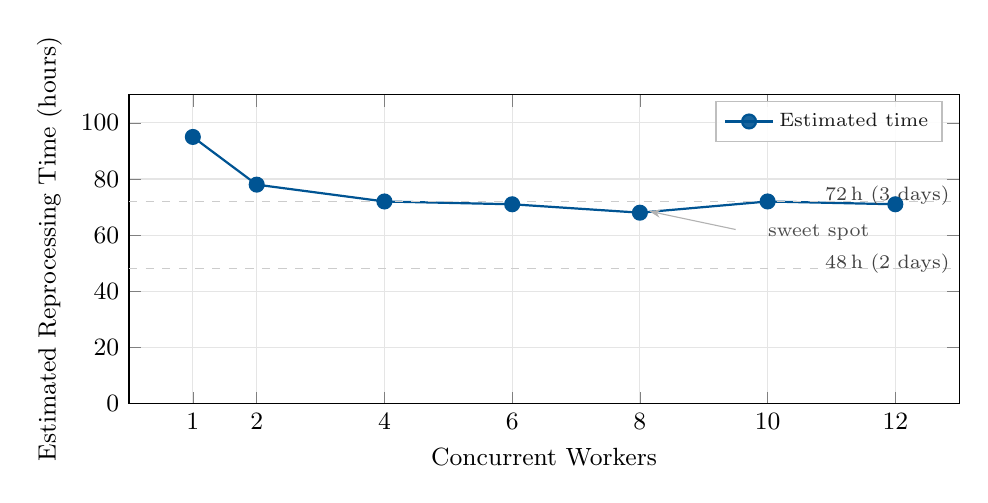
\begin{tikzpicture}
\begin{axis}[
  width=\columnwidth,
  height=5.5cm,
  xlabel={Concurrent Workers},
  ylabel={Estimated Reprocessing Time (hours)},
  xlabel style={font=\small},
  ylabel style={font=\small},
  xmin=0, xmax=13,
  ymin=0, ymax=110,
  xtick={1,2,4,6,8,10,12},
  ytick={0,20,40,60,80,100},
  yticklabel style={font=\small},
  xticklabel style={font=\small},
  grid=major,
  grid style={gray!20},
  legend style={font=\scriptsize, at={(0.98,0.98)}, anchor=north east,
    draw=gray!50, fill=white, fill opacity=0.9},
  every axis plot/.append style={thick},
]
% Measured
\addplot[ieeeblue, mark=*, mark size=2.5pt, mark options={solid, fill=ieeeblue}]
  coordinates {(1,95) (2,78) (4,72) (6,71) (8,68) (10,72) (12,71)};

% Reference lines
\draw[gray!40, dashed] (axis cs:0,72) -- (axis cs:13,72);
\node[font=\scriptsize, text=gray!50!black, anchor=east] at (axis cs:13,74) {72\,h (3 days)};
\draw[gray!40, dashed] (axis cs:0,48) -- (axis cs:13,48);
\node[font=\scriptsize, text=gray!50!black, anchor=east] at (axis cs:13,50) {48\,h (2 days)};

% Sweet spot
\draw[-{Stealth[length=4pt]}, gray!60] (axis cs:9.5,62) -- (axis cs:8.15,68.5);
\node[font=\scriptsize, text=gray!60!black] at (axis cs:10.8,61) {sweet spot};

\legend{Estimated time}
\end{axis}
\end{tikzpicture}
\caption{Reprocessing time for \num{3715} hours vs.\ concurrent workers.
  The sweet spot is 8 workers (68\,h). Beyond 8, VRAM saturation causes
  throughput to dip slightly, so the curve flattens rather than continuing
  to drop.}
\label{fig:projection}
\end{figure}

\subsection{Cost Comparison}

Table~\ref{tab:cost} puts the self-hosted numbers in context. For a corpus of
\num{3715} hours, cloud transcription costs range from roughly \$1,000 to
\$5,000. OpenTranscribe's cost is the hardware already on hand.

\begin{table}[!t]
\centering
\caption{Transcription Cost: Self-Hosted vs.\ Cloud (\num{3715} hours)}
\label{tab:cost}
\begin{tabular}{@{}lrrr@{}}
\toprule
\textbf{Provider} & \textbf{Rate/hr} & \textbf{Total} & \textbf{Speed} \\
\midrule
\textbf{OpenTranscribe} & \textbf{\$0} & \textbf{\$0} & 55$\times$ RT \\
Deepgram~\cite{deepgram2024}        & \$0.26 &   \$966  & $\sim$1$\times$ \\
OpenAI Whisper~\cite{openai2023gpt4}  & \$0.36 & \$1,337  & $\sim$1$\times$ \\
AssemblyAI~\cite{assemblyai2024}      & \$0.39 & \$1,449  & $\sim$1$\times$ \\
AWS Transcribe~\cite{amazontranscribe2024}  & \$1.44 & \$5,350  & $\sim$1$\times$ \\
\bottomrule
\end{tabular}
\\[4pt]
{\footnotesize Cloud rates as of March 2026 (standard tier, no volume
  discounts). Speed comparison is approximate---cloud APIs typically return
  results near 1$\times$ realtime. Self-hosted cost excludes hardware
  amortization and electricity.}
\end{table}

\subsection{Optimal Configuration}

Table~\ref{tab:optconfig} summarizes recommended configurations depending on
the deployment scenario.

\begin{table}[!t]
\centering
\caption{Recommended Deployment Configurations}
\label{tab:optconfig}
\begin{tabular}{@{}p{1.7cm}p{2.0cm}p{3.5cm}@{}}
\toprule
\textbf{Scenario} & \textbf{Config} & \textbf{Rationale} \\
\midrule
Production\newline (shared GPU) & conc=4--6 & Leaves VRAM for LLM, clustering, and other services \\
\addlinespace
Dedicated\newline reprocessing & conc=8 & Peak throughput (54.6$\times$); 44\,GB VRAM, 92\% of A6000 \\
\addlinespace
Maximum\newline capacity & conc=12 & Uses 99\% of VRAM; slightly lower throughput but 12$\times$ speedup \\
\bottomrule
\end{tabular}
\end{table}

% ==============================================================================
% X. HARDWARE RECOMMENDATIONS
% ==============================================================================
\section{Hardware Recommendations}

Table~\ref{tab:recommendations} maps GPU tiers to expected worker counts and
throughput. The estimates reflect the smaller batch sizes forced by less VRAM
and the measured throughput ceiling.

\begin{table}[!t]
\centering
\caption{GPU Tier Configuration Recommendations}
\label{tab:recommendations}
\begin{tabular}{@{}p{1.0cm}p{1.8cm}R{0.6cm}R{0.5cm}R{0.6cm}p{1.3cm}@{}}
\toprule
\textbf{Tier} & \textbf{GPUs} & \textbf{Max Wkr} & \textbf{Bat.} & \textbf{Thru.} & \textbf{Notes} \\
\midrule
4\,GB  & RTX 3050,\newline MX550          & 1 & 16 & see note & Whisper small; seq. \\
\addlinespace
6\,GB  & RTX 3060,\newline RTX 4050       & 1 & 16 & see note & Whisper medium; seq. \\
\addlinespace
8\,GB  & RTX 3070,\newline RTX 4060       & 1 & 16 & $\sim$30$\times$ & Whisper turbo; seq. \\
\addlinespace
12\,GB & RTX 3080\,Ti,\newline RTX 4070\,Ti & 2 & 16 & $\sim$38$\times$ & Limited concur. \\
\addlinespace
24\,GB & RTX 3090,\newline RTX 4090       & 4 & 16 & $\sim$47$\times$ & Full concur. \\
\addlinespace
48\,GB & RTX A6000,\newline A40           & 8--12 & 16 & $\sim$55$\times$ & Peak at conc=8;\newline 12 proven stable \\
\bottomrule
\end{tabular}
\\[4pt]
{\footnotesize Batch size shown is the Phase B ceiling; larger values buy no
  throughput (Fig.~\ref{fig:diar-throughput}). Set
  \texttt{DIARIZATION\_VRAM\_BUDGET\_MB} per-tier: \SI{1200}{} for
  \SI{4}{\giga\byte}, \SI{1500}{} for \SI{6}{\giga\byte}, unset for
  $\geq\!\SI{8}{\giga\byte}$. The 4--6\,GB tiers are throughput-unverified
  on dedicated hardware; numbers projected from the capped-A6000 whole-stack
  sweep at matching budgets.}
\end{table}

Practical takeaways:
\begin{itemize}[nosep,leftmargin=*]
  \item \textbf{4--6\,GB laptops now work.} Phase B's budget-aware batch
    selection drops the diarization footprint from \SI{5.7}{\giga\byte}
    (bs=64) to \SI{1.0}{\giga\byte} (bs=16) at identical accuracy, which
    lets Whisper small (\SI{0.75}{\giga\byte}) or medium
    (\SI{1.6}{\giga\byte}) coexist on a consumer laptop GPU. Set
    \texttt{DIARIZATION\_VRAM\_BUDGET\_MB=1200} on a \SI{4}{\giga\byte}
    card to leave room for Whisper.
  \item \textbf{24\,GB hits the ceiling.} Four workers fit, throughput maxes
    out at $\approx$47$\times$. The 48\,GB tier buys headroom for larger future
    models but does not increase throughput with the current pipeline.
  \item \textbf{Parallel diarization is now cheap.} At \SI{1}{\giga\byte}
    per pipeline, a single A6000 can host \SIrange{20}{25}{}
    concurrent diarizations, versus the one-at-a-time default in prior
    versions. Under-utilized in today's code but available for future
    multi-tenant deployments.
  \item \textbf{Buy a second GPU before a bigger one.} A 12\,GB card added
    alongside a 24\,GB card (5 workers total) beats a single 48\,GB card
    (4 workers, same throughput ceiling).
  \item \textbf{CPU-only does not work for diarization.} PyAnnote diarization
    times out after 10 minutes on a 30-minute file when forced onto CPU;
    the same file takes \SI{21}{\second} on GPU. Budget at least a
    \SI{4}{\giga\byte} card with the new policy.
\end{itemize}

% ==============================================================================
% X. CONCLUSION
% ==============================================================================
\section{Conclusion}

After fixing all GPU memory leaks, the true VRAM footprint turned out to be
remarkably small: 2.3\,GB peak for a single worker, or 4.7\% of the A6000.
Earlier measurements showed 9.4\,GB, but that included leaked CUDA contexts
from CPU worker processes---a finding that underscores the importance of clean
benchmarking baselines.

A single A6000 processes audio at 40.3$\times$ realtime (single file) and
sustains 35--39$\times$ across durations from 30\,minutes to 4\,hours.
Diarization and transcription split GPU time nearly evenly (50\% and 48\%),
with overhead at just 2\%. Concurrency scales linearly through 12 workers,
peaking at 54.6$\times$ aggregate throughput with 8 workers. Beyond 8, VRAM
saturation at $\approx$48.5\,GB causes slight throughput regression, but
scaling remains linear.

For the production corpus (\num{3715} hours, \num{1434} files), the sweet
spot of 8 concurrent workers finishes reprocessing in about 68 hours (2.8
days) at zero marginal cost---compared to \$966--\$5,350 for equivalent
cloud transcription.

The PyAnnote fork proved important both for the 1.28$\times$ speed gain and
for its constant VRAM footprint. Stock PyAnnote's unpredictable 7--17\,GB
spikes would have made high-concurrency VRAM budgeting unreliable.

Benchmarking surfaced several bugs: CPU workers silently creating CUDA
contexts (1.4\,GB each, 44\,GB total), batch size division starving the GPU
at high concurrency, and speaker assignment hiding a quadratic cost on long
files (80\,s $\to$ 6\,s after vectorization). A diarization embedding batch
size test showed minimal impact across batch=8/16/32---the fork's adaptive
sizing already picks the right value.

For future work, GPU-accelerated clustering (cuML) could reduce the
CPU-bound diarization fraction. Quality tiers (beam\_size=1 draft vs.\
beam\_size=5 production) would offer a 35\% speed option. And separating VAD
to a CPU preprocess stage could improve GPU utilization by 5--15\%.

\vspace{0.5em}
\noindent\textbf{Negative result: GPU-native Lance-Williams clustering.}\quad
We ported scipy's centroid-linkage Lance-Williams merge loop to pure PyTorch,
keeping the N$\times$N distance matrix, cluster centroids, and active-slot
mask resident on the A6000 through all N$-$1 merges. Correctness was
verified on fixed-seed synthetic blobs (11 parity tests against scipy).
On the real pyannote-community-1 workload (N$=$10{,}023 embeddings on the
2.2\,h reference), the GPU port ran in 14.2\,s versus scipy's ${\sim}$12\,s
---a slight regression. Root cause: the algorithm is intrinsically sequential
(each merge depends on the previous iteration's centroid update), and 10k
Python-level iterations at ${\sim}$1.5\,ms each of PyTorch dispatch overhead
offset the GPU math win. scipy's compiled C loop with cache-friendly array
access wins at this N on current hardware. The implementation ships as
opt-in infrastructure (\texttt{PYANNOTE\_ENABLE\_GPU\_LINKAGE=1}) for future
work: a \texttt{torch.jit.script} or fused CUDA kernel could amortize the
per-iteration overhead, and H100/B100-class hardware may tip the balance
through faster kernel launch latency. The broader lesson for future
optimization work: an algorithm's asymptotic complexity class doesn't tell
you where time is actually spent. Our Phase-3 pdist GPU port projected a
25--35\% end-to-end speedup on 4.7\,h based on ``clustering is 41\% of wall
time;'' measurement showed scipy's linkage was only ${\sim}$12\,s of that
138\,s stage, so an infinite-speedup linkage couldn't exceed an 8\% stage
gain. The rest of clustering is VBxClustering-specific CPU work (PLDA
re-scoring, AHC resolution search, twice-called \texttt{assign\_embeddings})
that would need stage-level restructuring to move off CPU.

\vspace{0.5em}
\noindent\textbf{Negative result: segmentation step reduction.}\quad
We tested reducing PyAnnote's default segmentation sliding-window overlap
from 90\% (\texttt{step=1.0\,s} over a 10\,s chunk) to 80\% and 70\%
(\texttt{step=2.0\,s}, \texttt{step=3.0\,s}). The wall-time
side behaved exactly as predicted: step=2.0 gave a 51\% end-to-end speedup
on the 2.2\,h reference and step=3.0 a 67\% speedup, because the segmentation
model processes proportionally fewer chunks and the downstream embedding and
clustering stages receive a smaller filtered set. DER on both configurations,
however, regressed beyond the 1.0\,pp opt-in gate (1.45\,pp at step=2.0,
1.73\,pp at step=3.0) with a speaker-count mismatch (3\,$\to$\,2 on the
reference file in both cases). The mechanism: PyAnnote's binarized segmentation
derives each frame's label from the average of every overlapping chunk's
posterior at that frame. At 90\% overlap a 2\,s turn by a minor speaker is
covered by \about{20} chunks; at 70\% overlap it's only 6, and if a few of
those happen to fall near the model's less-accurate chunk edges the averaged
posterior falls below the binarization threshold and the turn disappears
entirely. The speaker is then dropped from the downstream clustering, which
compounds into a full-pipeline speaker-count error. This failure mode is a
calibration-at-training-time artefact---PyAnnote was trained with 90\% overlap
and doesn't extrapolate gracefully. A retraining-style fix is out of scope
for this work, but the \texttt{segmentation\_step} knob remains available
for low-speaker-count inputs (interviews, monologues) where the short-turn-
degradation pathway doesn't apply.

% ==============================================================================
\vspace{0.5em}
\noindent\textbf{Availability.}\quad
OpenTranscribe is available at
\url{https://github.com/davidamacey/OpenTranscribe} under the AGPL-3.0 license.
The PyAnnote optimization fork is at
\url{https://github.com/davidamacey/pyannote-audio} (branch
\texttt{gpu-optimizations}).

\bibliographystyle{IEEEtran}
\bibliography{refs}

\end{document}
